\documentclass[11pt,a4paper]{article}
\usepackage[margin=1.9cm, top=2.1cm, bottom=2.0cm]{geometry}
\usepackage[T1]{fontenc}
\usepackage{lmodern}
\usepackage{amsmath,amssymb}
\usepackage{enumitem,booktabs,array,tabularx,multirow}
\usepackage[normalem]{ulem}
\usepackage{adjustbox}
\usepackage{xcolor}
\usepackage{fancyhdr,lastpage}
\usepackage[most]{tcolorbox}
\usepackage{tikz}
\usetikzlibrary{shapes.geometric,arrows.meta,positioning,calc}
\usepackage[hidelinks]{hyperref}
\setlength{\parindent}{0pt}
\setlength{\parskip}{4pt}
\renewcommand{\arraystretch}{1.25}
\emergencystretch=2em
\pagestyle{fancy}\fancyhf{}
\lhead{\small\textit{Course: CS420 -- Artificial Intelligence}}
\rhead{\small Practice Test 1 -- Solution}
\cfoot{\small Page \thepage\ of \pageref{LastPage}}
\renewcommand{\headrulewidth}{0.4pt}
% empty answer box (exam) / filled box (solution)
\newtcolorbox{ansbox}[1][]{enhanced, breakable, colback=white, colframe=black!55, boxrule=0.5pt, arc=0pt,
  left=5pt, right=5pt, top=3pt, bottom=3pt, before skip=3pt, after skip=6pt, #1}
\newtcolorbox{solbox}{enhanced, breakable, colback=blue!2!white, colframe=blue!50!black, boxrule=0.6pt, arc=0pt,
  left=6pt, right=6pt, top=4pt, bottom=4pt, before skip=3pt, after skip=8pt,
  fontupper=\color{black}}
\newcommand{\question}[1]{\par\medskip\noindent\textbf{Question #1.}\ }
\newcommand{\subq}[1]{\par\smallskip\noindent\textbf{#1}\ }
\newcommand{\T}{\textbf{\textcolor{green!45!black}{TRUE}}}
\newcommand{\F}{\textbf{\textcolor{red!70!black}{FALSE}}}

\tikzset{
  maxn/.style={draw, thick, regular polygon, regular polygon sides=3, minimum size=10.5mm, inner sep=0pt, font=\small},
  minn/.style={maxn, shape border rotate=180},
  chn/.style={draw, thick, circle, minimum size=9.5mm, inner sep=0pt, font=\small},
  leafn/.style={draw, rectangle, minimum width=5.5mm, minimum height=5.5mm, inner sep=1pt, font=\small},
  gone/.style={draw=black!25, text=black!35},
  cut/.style={red!80!black, very thick, dashed},
  sol/.style={text=blue!70!black, font=\small\bfseries},
}

\begin{document}


{\large\textbf{\textit{Course: CS420 -- Artificial Intelligence}}}\par
{\textbf{\textit{Midterm examination review -- Lectures 0 to 3}}}\par
\begin{center}{\Large\bfseries PRACTICE MIDTERM EXAMINATION -- TEST 1\\[2pt]\textcolor{blue!55!black}{SOLUTION}}\\[3pt]
{\small Duration: 120 minutes \quad$\cdot$\quad Closed book \quad$\cdot$\quad Calculator allowed}\end{center}
\noindent\rule{\linewidth}{0.6pt}

{\small\textit{Unless a question says otherwise, ties are broken in alphabetical order (left-to-right in trees), and successors are generated in alphabetical order.}}\par
\question{1}\textit{The two-jug problem.} You have a 4-litre jug and a 3-litre jug, both initially empty, and a tap with unlimited water. You may fill a jug from the tap, empty a jug onto the ground, or pour one jug into the other until the source is empty or the destination is full. The goal is to have \emph{exactly 2 litres in the 4-litre jug}.
\subq{(a)}Consider a state as a tuple of values. Which values should be included in the tuple?
\begin{solbox}
$(x, y)$: litres in the 4-L jug ($x\in\{0,\dots,4\}$) and in the 3-L jug ($y\in\{0,\dots,3\}$).
\end{solbox}
\subq{(b)}Define the initial state and the goal state(s).
\begin{solbox}
Initial $(0,0)$. Goal: any state with $x=2$, i.e.\ $(2,y)$ for $y=0..3$.
\end{solbox}
\subq{(c)}Define the action function (preconditions and effects of every action).
\begin{solbox}
Fill4: $x<4 \Rightarrow (4,y)$; Fill3: $y<3\Rightarrow(x,3)$; Empty4: $x>0\Rightarrow(0,y)$; Empty3: $y>0\Rightarrow(x,0)$; Pour4$\to$3: $x>0, y<3$, $t=\min(x,3-y)\Rightarrow(x-t,\,y+t)$; Pour3$\to$4: $y>0,x<4$, $t=\min(y,4-x)\Rightarrow(x+t,\,y-t)$.
\end{solbox}
\subq{(d)}What is the action cost?
\begin{solbox}
Each action costs 1 (path cost = number of actions).
\end{solbox}
\subq{(e)}What is the maximum number of states in the state space? How many are reachable from the initial state? Give a shortest solution.
\begin{solbox}
$5\times4=\mathbf{20}$ tuples. Reachable from $(0,0)$: \textbf{14} (every reachable state has at least one jug empty or full). Shortest solution (6 actions): (0,0) $\to$ (4,0) $\to$ (1,3) $\to$ (1,0) $\to$ (0,1) $\to$ (4,1) $\to$ (2,3).
\end{solbox}
\question{2}Consider the undirected graph below; $S$ is the initial state and $G$ the goal state. Step costs are written on the edges and the heuristic $h$ next to the vertices. \begin{center}
\begin{adjustbox}{max width=\linewidth}
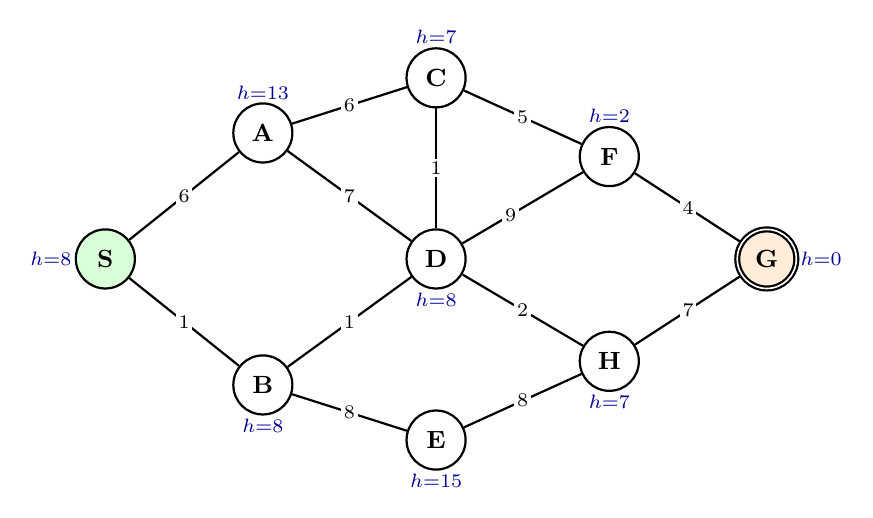
\begin{tikzpicture}[scale=1.0, every node/.style={transform shape}, gn/.style={draw, thick, circle, minimum size=7.5mm, inner sep=0pt, font=\small\bfseries}, ec/.style={font=\scriptsize, fill=white, inner sep=1pt}]
\node[gn, fill=green!15, label={[font=\scriptsize, text=blue!60!black, inner sep=1pt]left:$h{=}8$}] (S) at (0.00,0.00) {S};
\node[gn, label={[font=\scriptsize, text=blue!60!black, inner sep=1pt]above:$h{=}13$}] (A) at (2.00,1.60) {A};
\node[gn, label={[font=\scriptsize, text=blue!60!black, inner sep=1pt]below:$h{=}8$}] (B) at (2.00,-1.60) {B};
\node[gn, label={[font=\scriptsize, text=blue!60!black, inner sep=1pt]above:$h{=}7$}] (C) at (4.20,2.30) {C};
\node[gn, label={[font=\scriptsize, text=blue!60!black, inner sep=1pt]below:$h{=}8$}] (D) at (4.20,0.00) {D};
\node[gn, label={[font=\scriptsize, text=blue!60!black, inner sep=1pt]below:$h{=}15$}] (E) at (4.20,-2.30) {E};
\node[gn, label={[font=\scriptsize, text=blue!60!black, inner sep=1pt]above:$h{=}2$}] (F) at (6.40,1.30) {F};
\node[gn, label={[font=\scriptsize, text=blue!60!black, inner sep=1pt]below:$h{=}7$}] (H) at (6.40,-1.30) {H};
\node[gn, double, fill=orange!15, label={[font=\scriptsize, text=blue!60!black, inner sep=1pt]right:$h{=}0$}] (G) at (8.40,0.00) {G};
\draw[thick] (S) to[] node[ec, midway]{6} (A);
\draw[thick] (S) to[] node[ec, midway]{1} (B);
\draw[thick] (A) to[] node[ec, midway]{6} (C);
\draw[thick] (A) to[] node[ec, midway]{7} (D);
\draw[thick] (B) to[] node[ec, midway]{1} (D);
\draw[thick] (B) to[] node[ec, midway]{8} (E);
\draw[thick] (C) to[] node[ec, midway]{5} (F);
\draw[thick] (D) to[] node[ec, pos=0.4]{9} (F);
\draw[thick] (D) to[] node[ec, midway]{2} (H);
\draw[thick] (E) to[] node[ec, midway]{8} (H);
\draw[thick] (F) to[] node[ec, midway]{4} (G);
\draw[thick] (H) to[] node[ec, midway]{7} (G);
\draw[thick] (C) to[] node[ec, midway]{1} (D);
\end{tikzpicture}
\end{adjustbox}
\end{center}For each search strategy, (a) list, in order, the states \textbf{expanded}, (b) give the path found and (c) give the final content of the frontier (a state is expanded when it is removed from the frontier). Conventions: BFS, DFS and greedy best-first search test a state for the goal when it is \emph{generated} (so the goal is not expanded); UCS and A* test it when it is \emph{removed} from the frontier (graph search; a cheaper path to a frontier state replaces its entry). DFS avoids loops by remembering the states on the current path only. The path returned will not be accepted if the list of expanded states is wrong.

\begin{solbox}
\begin{center}\small\begin{tabularx}{\linewidth}{|>{\raggedright}p{2.6cm}|>{\raggedright}X|>{\raggedright}p{3.6cm}|>{\raggedright\arraybackslash}p{2.6cm}|}\hline
\textbf{Algorithm} & \textbf{List of expanded states} & \textbf{Path returned} & \textbf{Final frontier}\\ \hline
Breadth-first search & \textcolor{blue!60!black}{S A B C D E F} & \textcolor{blue!60!black}{S A C F G} (cost 21) & \textcolor{blue!60!black}{$\{$ H $\}$}\\ \hline
Uniform-cost search & \textcolor{blue!60!black}{S B D C H A F E G} & \textcolor{blue!60!black}{S B D H G} (cost 11) & \textcolor{blue!60!black}{$\{\ \}$}\\ \hline
Depth-first search & \textcolor{blue!60!black}{S A C D B E H} & \textcolor{blue!60!black}{S A C D B E H G} (cost 37) & \textcolor{blue!60!black}{(not asked)}\\ \hline
Greedy best-first search & \textcolor{blue!60!black}{S B D F} & \textcolor{blue!60!black}{S B D F G} (cost 15) & \textcolor{blue!60!black}{$\{$ C, H, A, E $\}$}\\ \hline
Graph-search A* & \textcolor{blue!60!black}{S B D C F H G} & \textcolor{blue!60!black}{S B D H G} (cost 11) & \textcolor{blue!60!black}{$\{$ A, E $\}$}\\ \hline
\end{tabularx}\end{center}\textbf{BFS} (queue after each expansion):\begin{center}\small\begin{tabularx}{\linewidth}{c c >{\raggedright\arraybackslash}X}\toprule
Step & Expanded & Queue (front $\rightarrow$ back) after the expansion \\ \midrule
1 & S & A, B \\
2 & A & B, C, D \\
3 & B & C, D, E \\
4 & C & D, E, F \\
5 & D & E, F, H \\
6 & E & F, H \\
7 & F & generates goal \textbf{G} $\Rightarrow$ stop; frontier: H \\
\bottomrule\end{tabularx}\end{center}\textbf{DFS} (stack after each expansion):\begin{center}\small\begin{tabularx}{\linewidth}{c c >{\raggedright\arraybackslash}X}\toprule
Step & Expanded & Stack (top $\rightarrow$ bottom) after the expansion \\ \midrule
1 & S & A, B \\
2 & A & C, D, B \\
3 & C & D, F, D, B \\
4 & D & B, F, H, F, D, B \\
5 & B & E, F, H, F, D, B \\
6 & E & H, F, H, F, D, B \\
7 & H & generates goal \textbf{G} $\Rightarrow$ stop; frontier: F, H, F, D, B \\
\bottomrule\end{tabularx}\end{center}\textbf{UCS:}\begin{center}\small\begin{tabularx}{\linewidth}{c l >{\raggedright\arraybackslash}X}\toprule
Step & Expanded & Frontier after the expansion, in priority order (subscript $=g(n)$) \\ \midrule
1 & S$_{0}$ & B$_{1}$, A$_{6}$ \\
2 & B$_{1}$ & D$_{2}$, A$_{6}$, E$_{9}$ \\
3 & D$_{2}$ & C$_{3}$, H$_{4}$, A$_{6}$, E$_{9}$, F$_{11}$ \\
4 & C$_{3}$ & H$_{4}$, A$_{6}$, F$_{8}$, E$_{9}$ \\
5 & H$_{4}$ & A$_{6}$, F$_{8}$, E$_{9}$, G$_{11}$ \\
6 & A$_{6}$ & F$_{8}$, E$_{9}$, G$_{11}$ \\
7 & F$_{8}$ & E$_{9}$, G$_{11}$ \\
8 & E$_{9}$ & G$_{11}$ \\
9 & G$_{11}$ & \textit{goal removed from the frontier -- stop} \\
\bottomrule\end{tabularx}\end{center}\textbf{Greedy best-first:}\begin{center}\small\begin{tabularx}{\linewidth}{c l >{\raggedright\arraybackslash}X}\toprule
Step & Expanded & Frontier after the expansion, in priority order (subscript $=h(n)$) \\ \midrule
1 & S$_{8}$ & B$_{8}$, A$_{13}$ \\
2 & B$_{8}$ & D$_{8}$, A$_{13}$, E$_{15}$ \\
3 & D$_{8}$ & F$_{2}$, C$_{7}$, H$_{7}$, A$_{13}$, E$_{15}$ \\
4 & F$_{2}$ & generates goal \textbf{G} $\Rightarrow$ stop; frontier: C$_{7}$, H$_{7}$, A$_{13}$, E$_{15}$ \\
\bottomrule\end{tabularx}\end{center}\textbf{A*:}\begin{center}\small\begin{tabularx}{\linewidth}{c l >{\raggedright\arraybackslash}X}\toprule
Step & Expanded & Frontier after the expansion, in priority order (subscript $=g+h=f$) \\ \midrule
1 & S$_{0+8=8}$ & B$_{1+8=9}$, A$_{6+13=19}$ \\
2 & B$_{1+8=9}$ & D$_{2+8=10}$, A$_{6+13=19}$, E$_{9+15=24}$ \\
3 & D$_{2+8=10}$ & C$_{3+7=10}$, H$_{4+7=11}$, F$_{11+2=13}$, A$_{6+13=19}$, E$_{9+15=24}$ \\
4 & C$_{3+7=10}$ & F$_{8+2=10}$, H$_{4+7=11}$, A$_{6+13=19}$, E$_{9+15=24}$ \\
5 & F$_{8+2=10}$ & H$_{4+7=11}$, G$_{12+0=12}$, A$_{6+13=19}$, E$_{9+15=24}$ \\
6 & H$_{4+7=11}$ & G$_{11+0=11}$, A$_{6+13=19}$, E$_{9+15=24}$ \\
7 & G$_{11+0=11}$ & \textit{goal removed from the frontier -- stop} \\
\bottomrule\end{tabularx}\end{center}
\end{solbox}
\subq{(d)}Is $h$ admissible? Justify.
\begin{solbox}
True costs $h^*$: S$=11$, A$=15$, B$=10$, C$=9$, D$=9$, E$=15$, F$=4$, H$=7$, G$=0$. $h(n)\le h^*(n)$ for every $n$ $\Rightarrow$ \textbf{admissible}.
\end{solbox}
\subq{(e)}Is $h$ consistent? Justify.
\begin{solbox}
$h(u)\le c(u,v)+h(v)$ holds on every edge in both directions (tight: $h(A)=c(A,C)+h(C)$, $h(C)=c(C,F)+h(F)$, $h(D)=c(D,C)+h(C)$, $h(E)=c(E,H)+h(H)$, $h(H)=c(H,G)+h(G)$) $\Rightarrow$ \textbf{consistent}.
\end{solbox}
\subq{(f)}Which of the five strategies returned an optimal path here, and which of them are guaranteed to do so?
\begin{solbox}
Optimal cost 11. UCS and A* found it; BFS (cost 21), DFS (37) and GBFS (15) did not. UCS (positive costs) and A* with an admissible/consistent heuristic are guaranteed optimal; BFS only when all step costs are equal; DFS and GBFS never.
\end{solbox}
\question{3}Consider the 8-puzzle. Apply \emph{steepest-descent hill climbing} with the Manhattan-distance heuristic $h$ to the following pair of initial and goal states.\begin{center}Initial state\quad \begin{tabular}{|c|c|c|}\hline 1 & 2 & 3\\\hline 6 & -- & 4\\\hline 8 & 7 & 5\\\hline\end{tabular}\qquad\qquad Goal state\quad \begin{tabular}{|c|c|c|}\hline 1 & 2 & 3\\\hline 8 & -- & 4\\\hline 7 & 6 & 5\\\hline\end{tabular}\end{center}Your work should: draw the search tree including all successors of every expanded state (moves of the blank in the order Up, Down, Left, Right; do not regenerate the parent state), write the heuristic value of every node, and mark the path found.
\par\smallskip\noindent 
\begin{solbox}
\begin{center}
\begin{adjustbox}{max width=\linewidth}
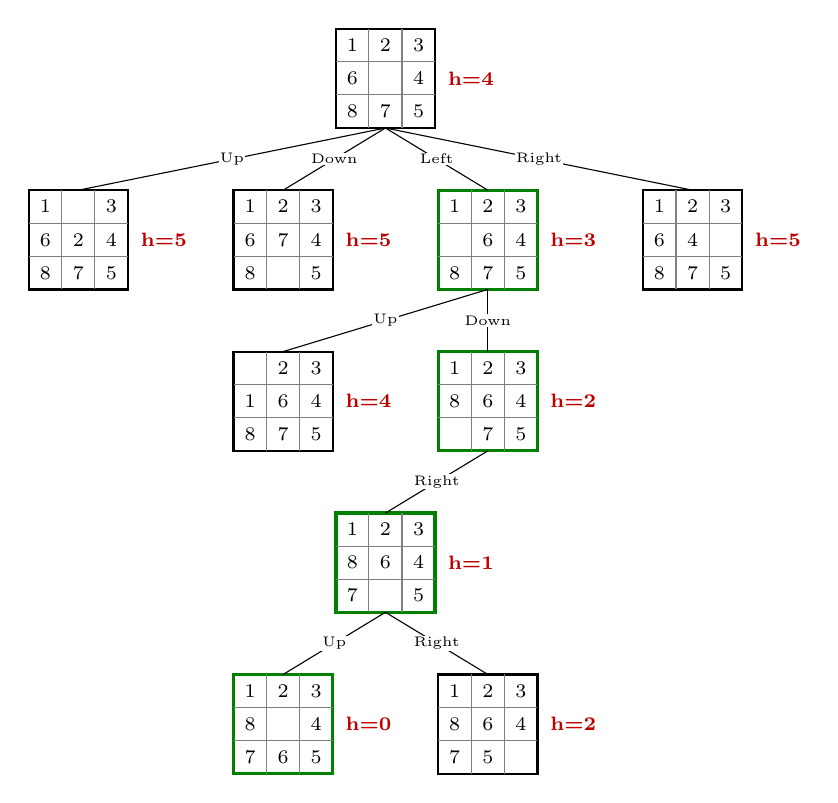
\begin{tikzpicture}
\draw[thick] (-0.63,0.00) rectangle (0.63,-1.26);
\draw[black!50] (-0.21,0.00) -- (-0.21,-1.26);
\draw[black!50] (-0.63,-0.42) -- (0.63,-0.42);
\draw[black!50] (0.21,0.00) -- (0.21,-1.26);
\draw[black!50] (-0.63,-0.84) -- (0.63,-0.84);
\node[font=\scriptsize] at (-0.42,-0.21) {1};
\node[font=\scriptsize] at (0.00,-0.21) {2};
\node[font=\scriptsize] at (0.42,-0.21) {3};
\node[font=\scriptsize] at (-0.42,-0.63) {6};
\node[font=\scriptsize] at (0.42,-0.63) {4};
\node[font=\scriptsize] at (-0.42,-1.05) {8};
\node[font=\scriptsize] at (0.00,-1.05) {7};
\node[font=\scriptsize] at (0.42,-1.05) {5};
\coordinate (r0-top) at (0.00,0.00);
\coordinate (r0-bot) at (0.00,-1.26);
\node[font=\scriptsize\bfseries, text=red!75!black, anchor=west] at (0.67,-0.63) {h=4};
\draw[thick] (-4.53,-2.05) rectangle (-3.27,-3.31);
\draw[black!50] (-4.11,-2.05) -- (-4.11,-3.31);
\draw[black!50] (-4.53,-2.47) -- (-3.27,-2.47);
\draw[black!50] (-3.69,-2.05) -- (-3.69,-3.31);
\draw[black!50] (-4.53,-2.89) -- (-3.27,-2.89);
\node[font=\scriptsize] at (-4.32,-2.26) {1};
\node[font=\scriptsize] at (-3.48,-2.26) {3};
\node[font=\scriptsize] at (-4.32,-2.68) {6};
\node[font=\scriptsize] at (-3.90,-2.68) {2};
\node[font=\scriptsize] at (-3.48,-2.68) {4};
\node[font=\scriptsize] at (-4.32,-3.10) {8};
\node[font=\scriptsize] at (-3.90,-3.10) {7};
\node[font=\scriptsize] at (-3.48,-3.10) {5};
\coordinate (b0_0-top) at (-3.90,-2.05);
\coordinate (b0_0-bot) at (-3.90,-3.31);
\node[font=\scriptsize\bfseries, text=red!75!black, anchor=west] at (-3.23,-2.68) {h=5};
\draw (r0-bot) -- node[font=\tiny, fill=white, inner sep=0.5pt]{Up} (b0_0-top);
\draw[thick] (-1.93,-2.05) rectangle (-0.67,-3.31);
\draw[black!50] (-1.51,-2.05) -- (-1.51,-3.31);
\draw[black!50] (-1.93,-2.47) -- (-0.67,-2.47);
\draw[black!50] (-1.09,-2.05) -- (-1.09,-3.31);
\draw[black!50] (-1.93,-2.89) -- (-0.67,-2.89);
\node[font=\scriptsize] at (-1.72,-2.26) {1};
\node[font=\scriptsize] at (-1.30,-2.26) {2};
\node[font=\scriptsize] at (-0.88,-2.26) {3};
\node[font=\scriptsize] at (-1.72,-2.68) {6};
\node[font=\scriptsize] at (-1.30,-2.68) {7};
\node[font=\scriptsize] at (-0.88,-2.68) {4};
\node[font=\scriptsize] at (-1.72,-3.10) {8};
\node[font=\scriptsize] at (-0.88,-3.10) {5};
\coordinate (b0_1-top) at (-1.30,-2.05);
\coordinate (b0_1-bot) at (-1.30,-3.31);
\node[font=\scriptsize\bfseries, text=red!75!black, anchor=west] at (-0.63,-2.68) {h=5};
\draw (r0-bot) -- node[font=\tiny, fill=white, inner sep=0.5pt]{Down} (b0_1-top);
\draw[very thick, draw=green!50!black] (0.67,-2.05) rectangle (1.93,-3.31);
\draw[black!50] (1.09,-2.05) -- (1.09,-3.31);
\draw[black!50] (0.67,-2.47) -- (1.93,-2.47);
\draw[black!50] (1.51,-2.05) -- (1.51,-3.31);
\draw[black!50] (0.67,-2.89) -- (1.93,-2.89);
\node[font=\scriptsize] at (0.88,-2.26) {1};
\node[font=\scriptsize] at (1.30,-2.26) {2};
\node[font=\scriptsize] at (1.72,-2.26) {3};
\node[font=\scriptsize] at (1.30,-2.68) {6};
\node[font=\scriptsize] at (1.72,-2.68) {4};
\node[font=\scriptsize] at (0.88,-3.10) {8};
\node[font=\scriptsize] at (1.30,-3.10) {7};
\node[font=\scriptsize] at (1.72,-3.10) {5};
\coordinate (b0_2-top) at (1.30,-2.05);
\coordinate (b0_2-bot) at (1.30,-3.31);
\node[font=\scriptsize\bfseries, text=red!75!black, anchor=west] at (1.97,-2.68) {h=3};
\draw (r0-bot) -- node[font=\tiny, fill=white, inner sep=0.5pt]{Left} (b0_2-top);
\draw[thick] (3.27,-2.05) rectangle (4.53,-3.31);
\draw[black!50] (3.69,-2.05) -- (3.69,-3.31);
\draw[black!50] (3.27,-2.47) -- (4.53,-2.47);
\draw[black!50] (4.11,-2.05) -- (4.11,-3.31);
\draw[black!50] (3.27,-2.89) -- (4.53,-2.89);
\node[font=\scriptsize] at (3.48,-2.26) {1};
\node[font=\scriptsize] at (3.90,-2.26) {2};
\node[font=\scriptsize] at (4.32,-2.26) {3};
\node[font=\scriptsize] at (3.48,-2.68) {6};
\node[font=\scriptsize] at (3.90,-2.68) {4};
\node[font=\scriptsize] at (3.48,-3.10) {8};
\node[font=\scriptsize] at (3.90,-3.10) {7};
\node[font=\scriptsize] at (4.32,-3.10) {5};
\coordinate (b0_3-top) at (3.90,-2.05);
\coordinate (b0_3-bot) at (3.90,-3.31);
\node[font=\scriptsize\bfseries, text=red!75!black, anchor=west] at (4.57,-2.68) {h=5};
\draw (r0-bot) -- node[font=\tiny, fill=white, inner sep=0.5pt]{Right} (b0_3-top);
\draw[thick] (-1.93,-4.10) rectangle (-0.67,-5.36);
\draw[black!50] (-1.51,-4.10) -- (-1.51,-5.36);
\draw[black!50] (-1.93,-4.52) -- (-0.67,-4.52);
\draw[black!50] (-1.09,-4.10) -- (-1.09,-5.36);
\draw[black!50] (-1.93,-4.94) -- (-0.67,-4.94);
\node[font=\scriptsize] at (-1.30,-4.31) {2};
\node[font=\scriptsize] at (-0.88,-4.31) {3};
\node[font=\scriptsize] at (-1.72,-4.73) {1};
\node[font=\scriptsize] at (-1.30,-4.73) {6};
\node[font=\scriptsize] at (-0.88,-4.73) {4};
\node[font=\scriptsize] at (-1.72,-5.15) {8};
\node[font=\scriptsize] at (-1.30,-5.15) {7};
\node[font=\scriptsize] at (-0.88,-5.15) {5};
\coordinate (b1_0-top) at (-1.30,-4.10);
\coordinate (b1_0-bot) at (-1.30,-5.36);
\node[font=\scriptsize\bfseries, text=red!75!black, anchor=west] at (-0.63,-4.73) {h=4};
\draw (b0_2-bot) -- node[font=\tiny, fill=white, inner sep=0.5pt]{Up} (b1_0-top);
\draw[very thick, draw=green!50!black] (0.67,-4.10) rectangle (1.93,-5.36);
\draw[black!50] (1.09,-4.10) -- (1.09,-5.36);
\draw[black!50] (0.67,-4.52) -- (1.93,-4.52);
\draw[black!50] (1.51,-4.10) -- (1.51,-5.36);
\draw[black!50] (0.67,-4.94) -- (1.93,-4.94);
\node[font=\scriptsize] at (0.88,-4.31) {1};
\node[font=\scriptsize] at (1.30,-4.31) {2};
\node[font=\scriptsize] at (1.72,-4.31) {3};
\node[font=\scriptsize] at (0.88,-4.73) {8};
\node[font=\scriptsize] at (1.30,-4.73) {6};
\node[font=\scriptsize] at (1.72,-4.73) {4};
\node[font=\scriptsize] at (1.30,-5.15) {7};
\node[font=\scriptsize] at (1.72,-5.15) {5};
\coordinate (b1_1-top) at (1.30,-4.10);
\coordinate (b1_1-bot) at (1.30,-5.36);
\node[font=\scriptsize\bfseries, text=red!75!black, anchor=west] at (1.97,-4.73) {h=2};
\draw (b0_2-bot) -- node[font=\tiny, fill=white, inner sep=0.5pt]{Down} (b1_1-top);
\draw[very thick, draw=green!50!black] (-0.63,-6.15) rectangle (0.63,-7.41);
\draw[black!50] (-0.21,-6.15) -- (-0.21,-7.41);
\draw[black!50] (-0.63,-6.57) -- (0.63,-6.57);
\draw[black!50] (0.21,-6.15) -- (0.21,-7.41);
\draw[black!50] (-0.63,-6.99) -- (0.63,-6.99);
\node[font=\scriptsize] at (-0.42,-6.36) {1};
\node[font=\scriptsize] at (0.00,-6.36) {2};
\node[font=\scriptsize] at (0.42,-6.36) {3};
\node[font=\scriptsize] at (-0.42,-6.78) {8};
\node[font=\scriptsize] at (0.00,-6.78) {6};
\node[font=\scriptsize] at (0.42,-6.78) {4};
\node[font=\scriptsize] at (-0.42,-7.20) {7};
\node[font=\scriptsize] at (0.42,-7.20) {5};
\coordinate (b2_0-top) at (0.00,-6.15);
\coordinate (b2_0-bot) at (0.00,-7.41);
\node[font=\scriptsize\bfseries, text=red!75!black, anchor=west] at (0.67,-6.78) {h=1};
\draw (b1_1-bot) -- node[font=\tiny, fill=white, inner sep=0.5pt]{Right} (b2_0-top);
\draw[very thick, draw=green!50!black] (-1.93,-8.20) rectangle (-0.67,-9.46);
\draw[black!50] (-1.51,-8.20) -- (-1.51,-9.46);
\draw[black!50] (-1.93,-8.62) -- (-0.67,-8.62);
\draw[black!50] (-1.09,-8.20) -- (-1.09,-9.46);
\draw[black!50] (-1.93,-9.04) -- (-0.67,-9.04);
\node[font=\scriptsize] at (-1.72,-8.41) {1};
\node[font=\scriptsize] at (-1.30,-8.41) {2};
\node[font=\scriptsize] at (-0.88,-8.41) {3};
\node[font=\scriptsize] at (-1.72,-8.83) {8};
\node[font=\scriptsize] at (-0.88,-8.83) {4};
\node[font=\scriptsize] at (-1.72,-9.25) {7};
\node[font=\scriptsize] at (-1.30,-9.25) {6};
\node[font=\scriptsize] at (-0.88,-9.25) {5};
\coordinate (b3_0-top) at (-1.30,-8.20);
\coordinate (b3_0-bot) at (-1.30,-9.46);
\node[font=\scriptsize\bfseries, text=red!75!black, anchor=west] at (-0.63,-8.83) {h=0};
\draw (b2_0-bot) -- node[font=\tiny, fill=white, inner sep=0.5pt]{Up} (b3_0-top);
\draw[thick] (0.67,-8.20) rectangle (1.93,-9.46);
\draw[black!50] (1.09,-8.20) -- (1.09,-9.46);
\draw[black!50] (0.67,-8.62) -- (1.93,-8.62);
\draw[black!50] (1.51,-8.20) -- (1.51,-9.46);
\draw[black!50] (0.67,-9.04) -- (1.93,-9.04);
\node[font=\scriptsize] at (0.88,-8.41) {1};
\node[font=\scriptsize] at (1.30,-8.41) {2};
\node[font=\scriptsize] at (1.72,-8.41) {3};
\node[font=\scriptsize] at (0.88,-8.83) {8};
\node[font=\scriptsize] at (1.30,-8.83) {6};
\node[font=\scriptsize] at (1.72,-8.83) {4};
\node[font=\scriptsize] at (0.88,-9.25) {7};
\node[font=\scriptsize] at (1.30,-9.25) {5};
\coordinate (b3_1-top) at (1.30,-8.20);
\coordinate (b3_1-bot) at (1.30,-9.46);
\node[font=\scriptsize\bfseries, text=red!75!black, anchor=west] at (1.97,-8.83) {h=2};
\draw (b2_0-bot) -- node[font=\tiny, fill=white, inner sep=0.5pt]{Right} (b3_1-top);
\end{tikzpicture}
\end{adjustbox}
\end{center}Each level keeps the successor with the smallest $h$ (green). $h$ decreases 4$\to$3$\to$2$\to$1$\to$0 and the goal is reached after 4 moves: Left, Down, Right, Up.
\end{solbox}
\question{4}Consider the following game tree. The root is a MAX node and the search always visits children left to right (small grey numbers are leaf indices).\begin{center}
\begin{adjustbox}{max width=\linewidth}
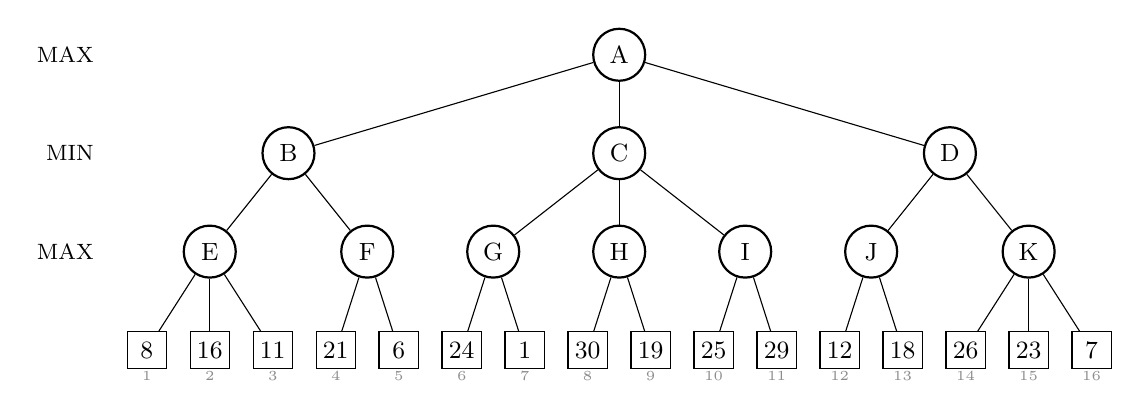
\begin{tikzpicture}[scale=1.0, every node/.style={transform shape}, gc/.style={draw, thick, circle, minimum size=6.6mm, inner sep=0pt, font=\small}, gl/.style={draw, rectangle, minimum width=5mm, minimum height=4.6mm, inner sep=1pt, font=\small}, gx/.style={draw=black!25, text=black!35}, val/.style={font=\footnotesize\bfseries, text=red!80!black, inner sep=1pt}]
\node[font=\footnotesize, anchor=east] at (-0.55,0.00) {MAX};
\node[font=\footnotesize, anchor=east] at (-0.55,-1.25) {MIN};
\node[font=\footnotesize, anchor=east] at (-0.55,-2.50) {MAX};
\node[gc] (n26) at (6.000,0.000) {A};
\node[gc] (n7) at (1.800,-1.250) {B};
\node[gc] (n3) at (0.800,-2.500) {E};
\node[gl, label={[font=\tiny, text=black!45, inner sep=1pt]below:1}] (n0) at (0.000,-3.750) {8};
\node[gl, label={[font=\tiny, text=black!45, inner sep=1pt]below:2}] (n1) at (0.800,-3.750) {16};
\node[gl, label={[font=\tiny, text=black!45, inner sep=1pt]below:3}] (n2) at (1.600,-3.750) {11};
\node[gc] (n6) at (2.800,-2.500) {F};
\node[gl, label={[font=\tiny, text=black!45, inner sep=1pt]below:4}] (n4) at (2.400,-3.750) {21};
\node[gl, label={[font=\tiny, text=black!45, inner sep=1pt]below:5}] (n5) at (3.200,-3.750) {6};
\node[gc] (n17) at (6.000,-1.250) {C};
\node[gc] (n10) at (4.400,-2.500) {G};
\node[gl, label={[font=\tiny, text=black!45, inner sep=1pt]below:6}] (n8) at (4.000,-3.750) {24};
\node[gl, label={[font=\tiny, text=black!45, inner sep=1pt]below:7}] (n9) at (4.800,-3.750) {1};
\node[gc] (n13) at (6.000,-2.500) {H};
\node[gl, label={[font=\tiny, text=black!45, inner sep=1pt]below:8}] (n11) at (5.600,-3.750) {30};
\node[gl, label={[font=\tiny, text=black!45, inner sep=1pt]below:9}] (n12) at (6.400,-3.750) {19};
\node[gc] (n16) at (7.600,-2.500) {I};
\node[gl, label={[font=\tiny, text=black!45, inner sep=1pt]below:10}] (n14) at (7.200,-3.750) {25};
\node[gl, label={[font=\tiny, text=black!45, inner sep=1pt]below:11}] (n15) at (8.000,-3.750) {29};
\node[gc] (n25) at (10.200,-1.250) {D};
\node[gc] (n20) at (9.200,-2.500) {J};
\node[gl, label={[font=\tiny, text=black!45, inner sep=1pt]below:12}] (n18) at (8.800,-3.750) {12};
\node[gl, label={[font=\tiny, text=black!45, inner sep=1pt]below:13}] (n19) at (9.600,-3.750) {18};
\node[gc] (n24) at (11.200,-2.500) {K};
\node[gl, label={[font=\tiny, text=black!45, inner sep=1pt]below:14}] (n21) at (10.400,-3.750) {26};
\node[gl, label={[font=\tiny, text=black!45, inner sep=1pt]below:15}] (n22) at (11.200,-3.750) {23};
\node[gl, label={[font=\tiny, text=black!45, inner sep=1pt]below:16}] (n23) at (12.000,-3.750) {7};
\draw (n26) -- (n7);
\draw (n26) -- (n17);
\draw (n26) -- (n25);
\draw (n7) -- (n3);
\draw (n7) -- (n6);
\draw (n3) -- (n0);
\draw (n3) -- (n1);
\draw (n3) -- (n2);
\draw (n6) -- (n4);
\draw (n6) -- (n5);
\draw (n17) -- (n10);
\draw (n17) -- (n13);
\draw (n17) -- (n16);
\draw (n10) -- (n8);
\draw (n10) -- (n9);
\draw (n13) -- (n11);
\draw (n13) -- (n12);
\draw (n16) -- (n14);
\draw (n16) -- (n15);
\draw (n25) -- (n20);
\draw (n25) -- (n24);
\draw (n20) -- (n18);
\draw (n20) -- (n19);
\draw (n24) -- (n21);
\draw (n24) -- (n22);
\draw (n24) -- (n23);
\end{tikzpicture}
\end{adjustbox}
\end{center}
\subq{(a)}Compute the final backed-up value of every node using the minimax algorithm (no alpha-beta pruning at this step). Which move should MAX make at the root?
\begin{solbox}
\begin{center}\small \begin{tabular}{|l|c|c|c|c|c|c|c|c|c|c|c|}\hline
\textbf{Node} & \textbf{A} & \textbf{B} & \textbf{C} & \textbf{D} & \textbf{E} & \textbf{F} & \textbf{G} & \textbf{H} & \textbf{I} & \textbf{J} & \textbf{K}\\ \hline
Minimax & \textcolor{blue!60!black}{24} & \textcolor{blue!60!black}{16} & \textcolor{blue!60!black}{24} & \textcolor{blue!60!black}{18} & \textcolor{blue!60!black}{16} & \textcolor{blue!60!black}{21} & \textcolor{blue!60!black}{24} & \textcolor{blue!60!black}{30} & \textcolor{blue!60!black}{29} & \textcolor{blue!60!black}{18} & \textcolor{blue!60!black}{26}\\[1.5mm] \hline
\end{tabular}\end{center}\begin{center}
\begin{adjustbox}{max width=\linewidth}
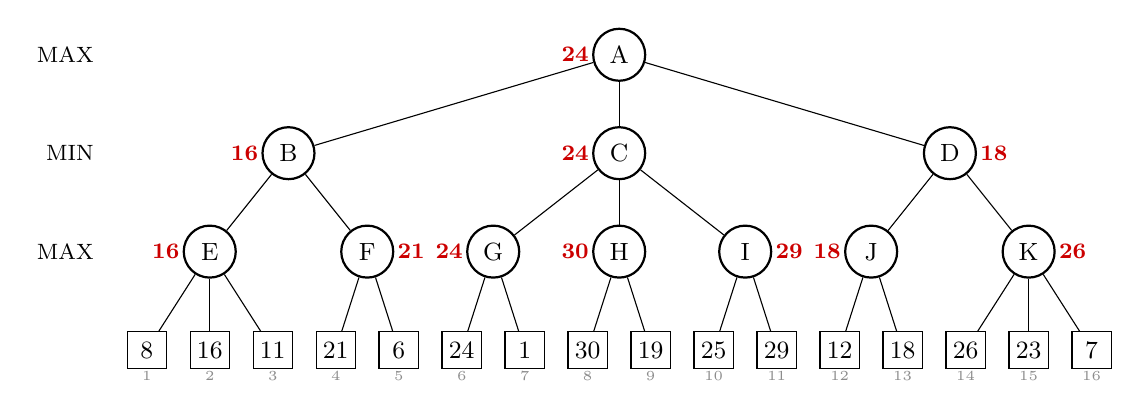
\begin{tikzpicture}[scale=1.0, every node/.style={transform shape}, gc/.style={draw, thick, circle, minimum size=6.6mm, inner sep=0pt, font=\small}, gl/.style={draw, rectangle, minimum width=5mm, minimum height=4.6mm, inner sep=1pt, font=\small}, gx/.style={draw=black!25, text=black!35}, val/.style={font=\footnotesize\bfseries, text=red!80!black, inner sep=1pt}]
\node[font=\footnotesize, anchor=east] at (-0.55,0.00) {MAX};
\node[font=\footnotesize, anchor=east] at (-0.55,-1.25) {MIN};
\node[font=\footnotesize, anchor=east] at (-0.55,-2.50) {MAX};
\node[gc, label={[val]left:24}] (n26) at (6.000,0.000) {A};
\node[gc, label={[val]left:16}] (n7) at (1.800,-1.250) {B};
\node[gc, label={[val]left:16}] (n3) at (0.800,-2.500) {E};
\node[gl, label={[font=\tiny, text=black!45, inner sep=1pt]below:1}] (n0) at (0.000,-3.750) {8};
\node[gl, label={[font=\tiny, text=black!45, inner sep=1pt]below:2}] (n1) at (0.800,-3.750) {16};
\node[gl, label={[font=\tiny, text=black!45, inner sep=1pt]below:3}] (n2) at (1.600,-3.750) {11};
\node[gc, label={[val]right:21}] (n6) at (2.800,-2.500) {F};
\node[gl, label={[font=\tiny, text=black!45, inner sep=1pt]below:4}] (n4) at (2.400,-3.750) {21};
\node[gl, label={[font=\tiny, text=black!45, inner sep=1pt]below:5}] (n5) at (3.200,-3.750) {6};
\node[gc, label={[val]left:24}] (n17) at (6.000,-1.250) {C};
\node[gc, label={[val]left:24}] (n10) at (4.400,-2.500) {G};
\node[gl, label={[font=\tiny, text=black!45, inner sep=1pt]below:6}] (n8) at (4.000,-3.750) {24};
\node[gl, label={[font=\tiny, text=black!45, inner sep=1pt]below:7}] (n9) at (4.800,-3.750) {1};
\node[gc, label={[val]left:30}] (n13) at (6.000,-2.500) {H};
\node[gl, label={[font=\tiny, text=black!45, inner sep=1pt]below:8}] (n11) at (5.600,-3.750) {30};
\node[gl, label={[font=\tiny, text=black!45, inner sep=1pt]below:9}] (n12) at (6.400,-3.750) {19};
\node[gc, label={[val]right:29}] (n16) at (7.600,-2.500) {I};
\node[gl, label={[font=\tiny, text=black!45, inner sep=1pt]below:10}] (n14) at (7.200,-3.750) {25};
\node[gl, label={[font=\tiny, text=black!45, inner sep=1pt]below:11}] (n15) at (8.000,-3.750) {29};
\node[gc, label={[val]right:18}] (n25) at (10.200,-1.250) {D};
\node[gc, label={[val]left:18}] (n20) at (9.200,-2.500) {J};
\node[gl, label={[font=\tiny, text=black!45, inner sep=1pt]below:12}] (n18) at (8.800,-3.750) {12};
\node[gl, label={[font=\tiny, text=black!45, inner sep=1pt]below:13}] (n19) at (9.600,-3.750) {18};
\node[gc, label={[val]right:26}] (n24) at (11.200,-2.500) {K};
\node[gl, label={[font=\tiny, text=black!45, inner sep=1pt]below:14}] (n21) at (10.400,-3.750) {26};
\node[gl, label={[font=\tiny, text=black!45, inner sep=1pt]below:15}] (n22) at (11.200,-3.750) {23};
\node[gl, label={[font=\tiny, text=black!45, inner sep=1pt]below:16}] (n23) at (12.000,-3.750) {7};
\draw (n26) -- (n7);
\draw (n26) -- (n17);
\draw (n26) -- (n25);
\draw (n7) -- (n3);
\draw (n7) -- (n6);
\draw (n3) -- (n0);
\draw (n3) -- (n1);
\draw (n3) -- (n2);
\draw (n6) -- (n4);
\draw (n6) -- (n5);
\draw (n17) -- (n10);
\draw (n17) -- (n13);
\draw (n17) -- (n16);
\draw (n10) -- (n8);
\draw (n10) -- (n9);
\draw (n13) -- (n11);
\draw (n13) -- (n12);
\draw (n16) -- (n14);
\draw (n16) -- (n15);
\draw (n25) -- (n20);
\draw (n25) -- (n24);
\draw (n20) -- (n18);
\draw (n20) -- (n19);
\draw (n24) -- (n21);
\draw (n24) -- (n22);
\draw (n24) -- (n23);
\end{tikzpicture}
\end{adjustbox}
\end{center}Root value $=24$; MAX moves to \textbf{C}.
\end{solbox}
\subq{(b)}Run alpha-beta pruning (children visited left to right). Give the value computed at every node (mark \textbf{X} if the node is never visited), cross out the pruned branches on the tree and briefly explain each case.
\begin{solbox}
\begin{center}\small \begin{tabular}{|l|c|c|c|c|c|c|c|c|c|c|c|}\hline
\textbf{Node} & \textbf{A} & \textbf{B} & \textbf{C} & \textbf{D} & \textbf{E} & \textbf{F} & \textbf{G} & \textbf{H} & \textbf{I} & \textbf{J} & \textbf{K}\\ \hline
$\alpha$-$\beta$ & \textcolor{blue!60!black}{$24$} & \textcolor{blue!60!black}{$16$} & \textcolor{blue!60!black}{$24$} & \textcolor{blue!60!black}{$\le 18$} & \textcolor{blue!60!black}{$16$} & \textcolor{blue!60!black}{$\ge 21$} & \textcolor{blue!60!black}{$24$} & \textcolor{blue!60!black}{$\ge 30$} & \textcolor{blue!60!black}{$\ge 25$} & \textcolor{blue!60!black}{$18$} & \textcolor{red!70!black}{\textbf{X}}\\[1.5mm] \hline
\end{tabular}\end{center}($\le v$ / $\ge v$: the node was cut off, so only this bound is known; writing the returned number $v$ is also accepted.)\begin{center}
\begin{adjustbox}{max width=\linewidth}
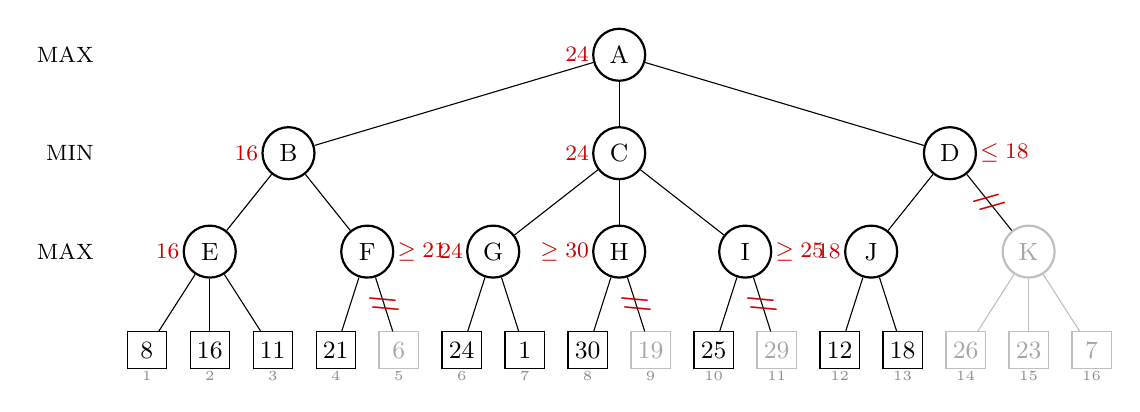
\begin{tikzpicture}[scale=1.0, every node/.style={transform shape}, gc/.style={draw, thick, circle, minimum size=6.6mm, inner sep=0pt, font=\small}, gl/.style={draw, rectangle, minimum width=5mm, minimum height=4.6mm, inner sep=1pt, font=\small}, gx/.style={draw=black!25, text=black!35}, val/.style={font=\footnotesize\bfseries, text=red!80!black, inner sep=1pt}]
\node[font=\footnotesize, anchor=east] at (-0.55,0.00) {MAX};
\node[font=\footnotesize, anchor=east] at (-0.55,-1.25) {MIN};
\node[font=\footnotesize, anchor=east] at (-0.55,-2.50) {MAX};
\node[gc, label={[val]left:$24$}] (n26) at (6.000,0.000) {A};
\node[gc, label={[val]left:$16$}] (n7) at (1.800,-1.250) {B};
\node[gc, label={[val]left:$16$}] (n3) at (0.800,-2.500) {E};
\node[gl, label={[font=\tiny, text=black!45, inner sep=1pt]below:1}] (n0) at (0.000,-3.750) {8};
\node[gl, label={[font=\tiny, text=black!45, inner sep=1pt]below:2}] (n1) at (0.800,-3.750) {16};
\node[gl, label={[font=\tiny, text=black!45, inner sep=1pt]below:3}] (n2) at (1.600,-3.750) {11};
\node[gc, label={[val]right:$\ge21$}] (n6) at (2.800,-2.500) {F};
\node[gl, label={[font=\tiny, text=black!45, inner sep=1pt]below:4}] (n4) at (2.400,-3.750) {21};
\node[gl, gx, label={[font=\tiny, text=black!45, inner sep=1pt]below:5}] (n5) at (3.200,-3.750) {6};
\node[gc, label={[val]left:$24$}] (n17) at (6.000,-1.250) {C};
\node[gc, label={[val]left:$24$}] (n10) at (4.400,-2.500) {G};
\node[gl, label={[font=\tiny, text=black!45, inner sep=1pt]below:6}] (n8) at (4.000,-3.750) {24};
\node[gl, label={[font=\tiny, text=black!45, inner sep=1pt]below:7}] (n9) at (4.800,-3.750) {1};
\node[gc, label={[val]left:$\ge30$}] (n13) at (6.000,-2.500) {H};
\node[gl, label={[font=\tiny, text=black!45, inner sep=1pt]below:8}] (n11) at (5.600,-3.750) {30};
\node[gl, gx, label={[font=\tiny, text=black!45, inner sep=1pt]below:9}] (n12) at (6.400,-3.750) {19};
\node[gc, label={[val]right:$\ge25$}] (n16) at (7.600,-2.500) {I};
\node[gl, label={[font=\tiny, text=black!45, inner sep=1pt]below:10}] (n14) at (7.200,-3.750) {25};
\node[gl, gx, label={[font=\tiny, text=black!45, inner sep=1pt]below:11}] (n15) at (8.000,-3.750) {29};
\node[gc, label={[val]right:$\le18$}] (n25) at (10.200,-1.250) {D};
\node[gc, label={[val]left:$18$}] (n20) at (9.200,-2.500) {J};
\node[gl, label={[font=\tiny, text=black!45, inner sep=1pt]below:12}] (n18) at (8.800,-3.750) {12};
\node[gl, label={[font=\tiny, text=black!45, inner sep=1pt]below:13}] (n19) at (9.600,-3.750) {18};
\node[gc, gx] (n24) at (11.200,-2.500) {K};
\node[gl, gx, label={[font=\tiny, text=black!45, inner sep=1pt]below:14}] (n21) at (10.400,-3.750) {26};
\node[gl, gx, label={[font=\tiny, text=black!45, inner sep=1pt]below:15}] (n22) at (11.200,-3.750) {23};
\node[gl, gx, label={[font=\tiny, text=black!45, inner sep=1pt]below:16}] (n23) at (12.000,-3.750) {7};
\draw (n26) -- (n7);
\draw (n26) -- (n17);
\draw (n26) -- (n25);
\draw (n7) -- (n3);
\draw (n7) -- (n6);
\draw (n3) -- (n0);
\draw (n3) -- (n1);
\draw (n3) -- (n2);
\draw (n6) -- (n4);
\draw (n6) -- (n5) node[midway, sloped, text=red!80!black, font=\small\bfseries, inner sep=0pt]{/\!/};
\draw (n17) -- (n10);
\draw (n17) -- (n13);
\draw (n17) -- (n16);
\draw (n10) -- (n8);
\draw (n10) -- (n9);
\draw (n13) -- (n11);
\draw (n13) -- (n12) node[midway, sloped, text=red!80!black, font=\small\bfseries, inner sep=0pt]{/\!/};
\draw (n16) -- (n14);
\draw (n16) -- (n15) node[midway, sloped, text=red!80!black, font=\small\bfseries, inner sep=0pt]{/\!/};
\draw (n25) -- (n20);
\draw (n25) -- (n24) node[midway, sloped, text=red!80!black, font=\small\bfseries, inner sep=0pt]{/\!/};
\draw (n20) -- (n18);
\draw (n20) -- (n19);
\draw[black!25] (n24) -- (n21);
\draw[black!25] (n24) -- (n22);
\draw[black!25] (n24) -- (n23);
\end{tikzpicture}
\end{adjustbox}
\end{center}$\alpha$ and $\beta$ at every visited node:\begin{center}\small\begin{tabular}{c c c c c}\toprule Node & Type & On entry & When it returns & Value returned\\\midrule A & MAX & $\alpha=-\infty,\ \beta=+\infty$ & $\alpha=24,\ \beta=+\infty$ & $24$ \\
B & MIN & $\alpha=-\infty,\ \beta=+\infty$ & $\alpha=-\infty,\ \beta=16$ & $16$ \\
E & MAX & $\alpha=-\infty,\ \beta=+\infty$ & $\alpha=16,\ \beta=+\infty$ & $16$ \\
F & MAX & $\alpha=-\infty,\ \beta=16$ & $\alpha=21,\ \beta=16$ & $\ge 21$ \\
C & MIN & $\alpha=16,\ \beta=+\infty$ & $\alpha=16,\ \beta=24$ & $24$ \\
G & MAX & $\alpha=16,\ \beta=+\infty$ & $\alpha=24,\ \beta=+\infty$ & $24$ \\
H & MAX & $\alpha=16,\ \beta=24$ & $\alpha=30,\ \beta=24$ & $\ge 30$ \\
I & MAX & $\alpha=16,\ \beta=24$ & $\alpha=25,\ \beta=24$ & $\ge 25$ \\
D & MIN & $\alpha=24,\ \beta=+\infty$ & $\alpha=24,\ \beta=18$ & $\le 18$ \\
J & MAX & $\alpha=24,\ \beta=+\infty$ & $\alpha=24,\ \beta=+\infty$ & $18$ \\\bottomrule\end{tabular}\end{center}\begin{itemize}[leftmargin=1.5em,itemsep=1pt]
\item At MAX node \textbf{F}, after leaf \#4: $v=21 \ge \beta=16$ $\Rightarrow$ prune leaf \#5. (MIN at B already has an alternative worth $\beta=16$, so it will never let play reach F.)
\item At MAX node \textbf{H}, after leaf \#8: $v=30 \ge \beta=24$ $\Rightarrow$ prune leaf \#9. (MIN at C already has an alternative worth $\beta=24$, so it will never let play reach H.)
\item At MAX node \textbf{I}, after leaf \#10: $v=25 \ge \beta=24$ $\Rightarrow$ prune leaf \#11. (MIN at C already has an alternative worth $\beta=24$, so it will never let play reach I.)
\item At MIN node \textbf{D}, after child J: $v=18 \le \alpha=24$ $\Rightarrow$ prune K (leaves \#14--\#16). (MAX at A already has an alternative worth $\alpha=24$, so it will never let play reach D.)
\end{itemize}Leaves evaluated: 10 of 16.
\end{solbox}
\subq{(c)}Using the minimax values from (a), and without performing any alpha-beta calculation, rotate the children of each node at every level so that alpha-beta prunes as much as possible. Draw the new tree (keep the node letters).
\begin{solbox}
Best child first for the player to move (MAX: largest value first, MIN: smallest first):\begin{center}
\begin{adjustbox}{max width=\linewidth}
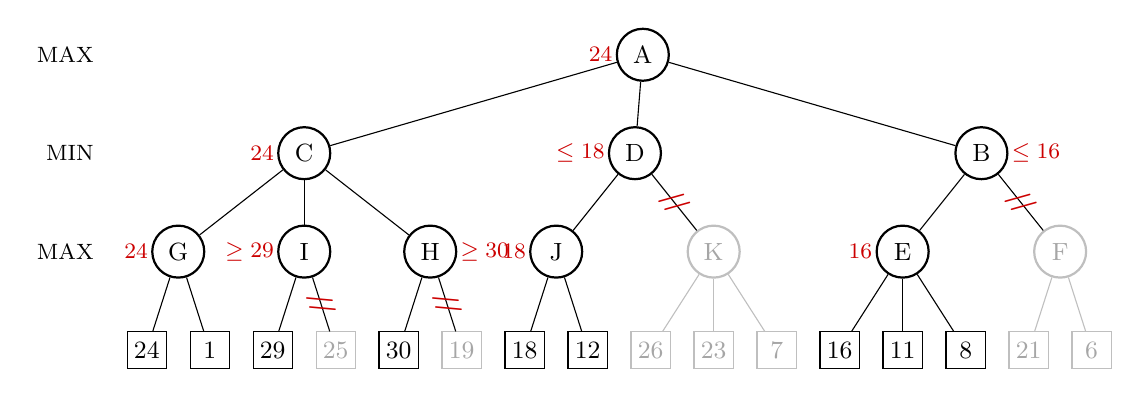
\begin{tikzpicture}[scale=1.0, every node/.style={transform shape}, gc/.style={draw, thick, circle, minimum size=6.6mm, inner sep=0pt, font=\small}, gl/.style={draw, rectangle, minimum width=5mm, minimum height=4.6mm, inner sep=1pt, font=\small}, gx/.style={draw=black!25, text=black!35}, val/.style={font=\footnotesize\bfseries, text=red!80!black, inner sep=1pt}]
\node[font=\footnotesize, anchor=east] at (-0.55,0.00) {MAX};
\node[font=\footnotesize, anchor=east] at (-0.55,-1.25) {MIN};
\node[font=\footnotesize, anchor=east] at (-0.55,-2.50) {MAX};
\node[gc, label={[val]left:$24$}] (n26) at (6.300,0.000) {A};
\node[gc, label={[val]left:$24$}] (n9) at (2.000,-1.250) {C};
\node[gc, label={[val]left:$24$}] (n2) at (0.400,-2.500) {G};
\node[gl] (n0) at (0.000,-3.750) {24};
\node[gl] (n1) at (0.800,-3.750) {1};
\node[gc, label={[val]left:$\ge29$}] (n5) at (2.000,-2.500) {I};
\node[gl] (n3) at (1.600,-3.750) {29};
\node[gl, gx] (n4) at (2.400,-3.750) {25};
\node[gc, label={[val]right:$\ge30$}] (n8) at (3.600,-2.500) {H};
\node[gl] (n6) at (3.200,-3.750) {30};
\node[gl, gx] (n7) at (4.000,-3.750) {19};
\node[gc, label={[val]left:$\le18$}] (n17) at (6.200,-1.250) {D};
\node[gc, label={[val]left:$18$}] (n12) at (5.200,-2.500) {J};
\node[gl] (n10) at (4.800,-3.750) {18};
\node[gl] (n11) at (5.600,-3.750) {12};
\node[gc, gx] (n16) at (7.200,-2.500) {K};
\node[gl, gx] (n13) at (6.400,-3.750) {26};
\node[gl, gx] (n14) at (7.200,-3.750) {23};
\node[gl, gx] (n15) at (8.000,-3.750) {7};
\node[gc, label={[val]right:$\le16$}] (n25) at (10.600,-1.250) {B};
\node[gc, label={[val]left:$16$}] (n21) at (9.600,-2.500) {E};
\node[gl] (n18) at (8.800,-3.750) {16};
\node[gl] (n19) at (9.600,-3.750) {11};
\node[gl] (n20) at (10.400,-3.750) {8};
\node[gc, gx] (n24) at (11.600,-2.500) {F};
\node[gl, gx] (n22) at (11.200,-3.750) {21};
\node[gl, gx] (n23) at (12.000,-3.750) {6};
\draw (n26) -- (n9);
\draw (n26) -- (n17);
\draw (n26) -- (n25);
\draw (n9) -- (n2);
\draw (n9) -- (n5);
\draw (n9) -- (n8);
\draw (n2) -- (n0);
\draw (n2) -- (n1);
\draw (n5) -- (n3);
\draw (n5) -- (n4) node[midway, sloped, text=red!80!black, font=\small\bfseries, inner sep=0pt]{/\!/};
\draw (n8) -- (n6);
\draw (n8) -- (n7) node[midway, sloped, text=red!80!black, font=\small\bfseries, inner sep=0pt]{/\!/};
\draw (n17) -- (n12);
\draw (n17) -- (n16) node[midway, sloped, text=red!80!black, font=\small\bfseries, inner sep=0pt]{/\!/};
\draw (n12) -- (n10);
\draw (n12) -- (n11);
\draw[black!25] (n16) -- (n13);
\draw[black!25] (n16) -- (n14);
\draw[black!25] (n16) -- (n15);
\draw (n25) -- (n21);
\draw (n25) -- (n24) node[midway, sloped, text=red!80!black, font=\small\bfseries, inner sep=0pt]{/\!/};
\draw (n21) -- (n18);
\draw (n21) -- (n19);
\draw (n21) -- (n20);
\draw[black!25] (n24) -- (n22);
\draw[black!25] (n24) -- (n23);
\end{tikzpicture}
\end{adjustbox}
\end{center}With this ordering alpha-beta evaluates only \textbf{9} leaves (instead of 10).
\end{solbox}
\question{5}Consider the following 4-ply game tree (MAX at the root).\begin{center}
\begin{adjustbox}{max width=\linewidth}
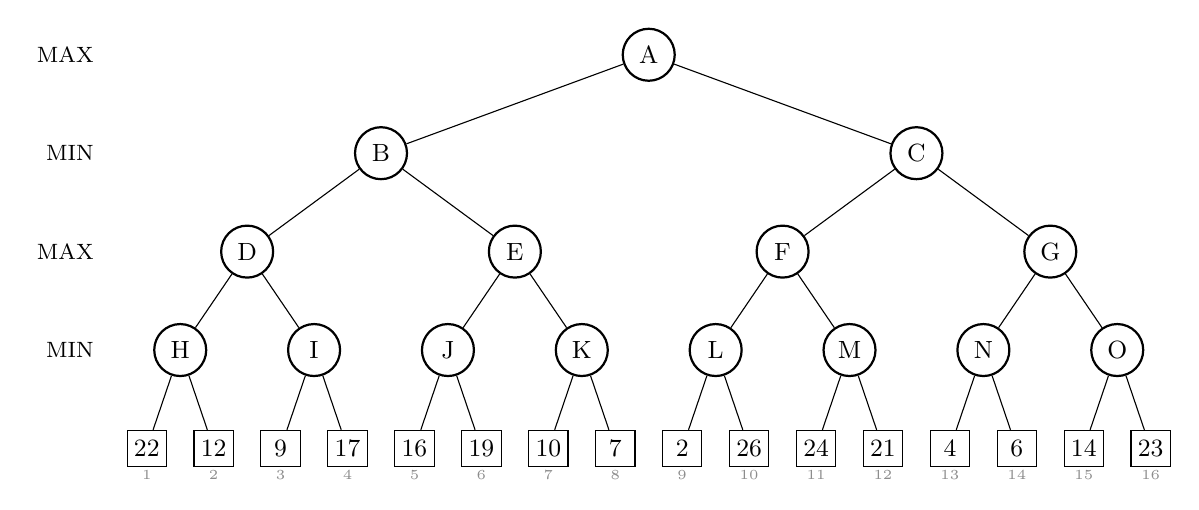
\begin{tikzpicture}[scale=1.0, every node/.style={transform shape}, gc/.style={draw, thick, circle, minimum size=6.6mm, inner sep=0pt, font=\small}, gl/.style={draw, rectangle, minimum width=5mm, minimum height=4.6mm, inner sep=1pt, font=\small}, gx/.style={draw=black!25, text=black!35}, val/.style={font=\footnotesize\bfseries, text=red!80!black, inner sep=1pt}]
\node[font=\footnotesize, anchor=east] at (-0.55,0.00) {MAX};
\node[font=\footnotesize, anchor=east] at (-0.55,-1.25) {MIN};
\node[font=\footnotesize, anchor=east] at (-0.55,-2.50) {MAX};
\node[font=\footnotesize, anchor=east] at (-0.55,-3.75) {MIN};
\node[gc] (n30) at (6.375,0.000) {A};
\node[gc] (n14) at (2.975,-1.250) {B};
\node[gc] (n6) at (1.275,-2.500) {D};
\node[gc] (n2) at (0.425,-3.750) {H};
\node[gl, label={[font=\tiny, text=black!45, inner sep=1pt]below:1}] (n0) at (0.000,-5.000) {22};
\node[gl, label={[font=\tiny, text=black!45, inner sep=1pt]below:2}] (n1) at (0.850,-5.000) {12};
\node[gc] (n5) at (2.125,-3.750) {I};
\node[gl, label={[font=\tiny, text=black!45, inner sep=1pt]below:3}] (n3) at (1.700,-5.000) {9};
\node[gl, label={[font=\tiny, text=black!45, inner sep=1pt]below:4}] (n4) at (2.550,-5.000) {17};
\node[gc] (n13) at (4.675,-2.500) {E};
\node[gc] (n9) at (3.825,-3.750) {J};
\node[gl, label={[font=\tiny, text=black!45, inner sep=1pt]below:5}] (n7) at (3.400,-5.000) {16};
\node[gl, label={[font=\tiny, text=black!45, inner sep=1pt]below:6}] (n8) at (4.250,-5.000) {19};
\node[gc] (n12) at (5.525,-3.750) {K};
\node[gl, label={[font=\tiny, text=black!45, inner sep=1pt]below:7}] (n10) at (5.100,-5.000) {10};
\node[gl, label={[font=\tiny, text=black!45, inner sep=1pt]below:8}] (n11) at (5.950,-5.000) {7};
\node[gc] (n29) at (9.775,-1.250) {C};
\node[gc] (n21) at (8.075,-2.500) {F};
\node[gc] (n17) at (7.225,-3.750) {L};
\node[gl, label={[font=\tiny, text=black!45, inner sep=1pt]below:9}] (n15) at (6.800,-5.000) {2};
\node[gl, label={[font=\tiny, text=black!45, inner sep=1pt]below:10}] (n16) at (7.650,-5.000) {26};
\node[gc] (n20) at (8.925,-3.750) {M};
\node[gl, label={[font=\tiny, text=black!45, inner sep=1pt]below:11}] (n18) at (8.500,-5.000) {24};
\node[gl, label={[font=\tiny, text=black!45, inner sep=1pt]below:12}] (n19) at (9.350,-5.000) {21};
\node[gc] (n28) at (11.475,-2.500) {G};
\node[gc] (n24) at (10.625,-3.750) {N};
\node[gl, label={[font=\tiny, text=black!45, inner sep=1pt]below:13}] (n22) at (10.200,-5.000) {4};
\node[gl, label={[font=\tiny, text=black!45, inner sep=1pt]below:14}] (n23) at (11.050,-5.000) {6};
\node[gc] (n27) at (12.325,-3.750) {O};
\node[gl, label={[font=\tiny, text=black!45, inner sep=1pt]below:15}] (n25) at (11.900,-5.000) {14};
\node[gl, label={[font=\tiny, text=black!45, inner sep=1pt]below:16}] (n26) at (12.750,-5.000) {23};
\draw (n30) -- (n14);
\draw (n30) -- (n29);
\draw (n14) -- (n6);
\draw (n14) -- (n13);
\draw (n6) -- (n2);
\draw (n6) -- (n5);
\draw (n2) -- (n0);
\draw (n2) -- (n1);
\draw (n5) -- (n3);
\draw (n5) -- (n4);
\draw (n13) -- (n9);
\draw (n13) -- (n12);
\draw (n9) -- (n7);
\draw (n9) -- (n8);
\draw (n12) -- (n10);
\draw (n12) -- (n11);
\draw (n29) -- (n21);
\draw (n29) -- (n28);
\draw (n21) -- (n17);
\draw (n21) -- (n20);
\draw (n17) -- (n15);
\draw (n17) -- (n16);
\draw (n20) -- (n18);
\draw (n20) -- (n19);
\draw (n28) -- (n24);
\draw (n28) -- (n27);
\draw (n24) -- (n22);
\draw (n24) -- (n23);
\draw (n27) -- (n25);
\draw (n27) -- (n26);
\end{tikzpicture}
\end{adjustbox}
\end{center}
\subq{(a)}Note the minimax value of every node (no pruning).
\begin{solbox}
\begin{center}\small \begin{tabular}{|l|c|c|c|c|c|c|c|c|c|c|c|c|c|c|c|}\hline
\textbf{Node} & \textbf{A} & \textbf{B} & \textbf{C} & \textbf{D} & \textbf{E} & \textbf{F} & \textbf{G} & \textbf{H} & \textbf{I} & \textbf{J} & \textbf{K} & \textbf{L} & \textbf{M} & \textbf{N} & \textbf{O}\\ \hline
Minimax & \textcolor{blue!60!black}{14} & \textcolor{blue!60!black}{12} & \textcolor{blue!60!black}{14} & \textcolor{blue!60!black}{12} & \textcolor{blue!60!black}{16} & \textcolor{blue!60!black}{21} & \textcolor{blue!60!black}{14} & \textcolor{blue!60!black}{12} & \textcolor{blue!60!black}{9} & \textcolor{blue!60!black}{16} & \textcolor{blue!60!black}{7} & \textcolor{blue!60!black}{2} & \textcolor{blue!60!black}{21} & \textcolor{blue!60!black}{4} & \textcolor{blue!60!black}{14}\\[1.5mm] \hline
\end{tabular}\end{center}Root value $=14$; MAX moves to \textbf{C}.
\end{solbox}
\subq{(b)}Show where alpha-beta pruning occurs (left to right) by crossing out the corresponding branches, and briefly explain each case.
\begin{solbox}
\begin{center}
\begin{adjustbox}{max width=\linewidth}
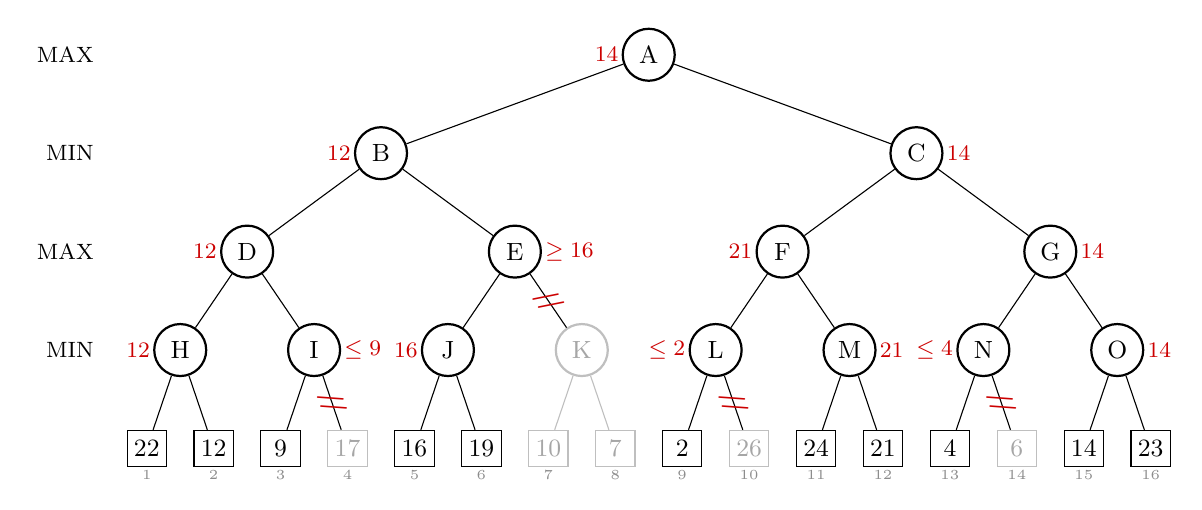
\begin{tikzpicture}[scale=1.0, every node/.style={transform shape}, gc/.style={draw, thick, circle, minimum size=6.6mm, inner sep=0pt, font=\small}, gl/.style={draw, rectangle, minimum width=5mm, minimum height=4.6mm, inner sep=1pt, font=\small}, gx/.style={draw=black!25, text=black!35}, val/.style={font=\footnotesize\bfseries, text=red!80!black, inner sep=1pt}]
\node[font=\footnotesize, anchor=east] at (-0.55,0.00) {MAX};
\node[font=\footnotesize, anchor=east] at (-0.55,-1.25) {MIN};
\node[font=\footnotesize, anchor=east] at (-0.55,-2.50) {MAX};
\node[font=\footnotesize, anchor=east] at (-0.55,-3.75) {MIN};
\node[gc, label={[val]left:$14$}] (n30) at (6.375,0.000) {A};
\node[gc, label={[val]left:$12$}] (n14) at (2.975,-1.250) {B};
\node[gc, label={[val]left:$12$}] (n6) at (1.275,-2.500) {D};
\node[gc, label={[val]left:$12$}] (n2) at (0.425,-3.750) {H};
\node[gl, label={[font=\tiny, text=black!45, inner sep=1pt]below:1}] (n0) at (0.000,-5.000) {22};
\node[gl, label={[font=\tiny, text=black!45, inner sep=1pt]below:2}] (n1) at (0.850,-5.000) {12};
\node[gc, label={[val]right:$\le9$}] (n5) at (2.125,-3.750) {I};
\node[gl, label={[font=\tiny, text=black!45, inner sep=1pt]below:3}] (n3) at (1.700,-5.000) {9};
\node[gl, gx, label={[font=\tiny, text=black!45, inner sep=1pt]below:4}] (n4) at (2.550,-5.000) {17};
\node[gc, label={[val]right:$\ge16$}] (n13) at (4.675,-2.500) {E};
\node[gc, label={[val]left:$16$}] (n9) at (3.825,-3.750) {J};
\node[gl, label={[font=\tiny, text=black!45, inner sep=1pt]below:5}] (n7) at (3.400,-5.000) {16};
\node[gl, label={[font=\tiny, text=black!45, inner sep=1pt]below:6}] (n8) at (4.250,-5.000) {19};
\node[gc, gx] (n12) at (5.525,-3.750) {K};
\node[gl, gx, label={[font=\tiny, text=black!45, inner sep=1pt]below:7}] (n10) at (5.100,-5.000) {10};
\node[gl, gx, label={[font=\tiny, text=black!45, inner sep=1pt]below:8}] (n11) at (5.950,-5.000) {7};
\node[gc, label={[val]right:$14$}] (n29) at (9.775,-1.250) {C};
\node[gc, label={[val]left:$21$}] (n21) at (8.075,-2.500) {F};
\node[gc, label={[val]left:$\le2$}] (n17) at (7.225,-3.750) {L};
\node[gl, label={[font=\tiny, text=black!45, inner sep=1pt]below:9}] (n15) at (6.800,-5.000) {2};
\node[gl, gx, label={[font=\tiny, text=black!45, inner sep=1pt]below:10}] (n16) at (7.650,-5.000) {26};
\node[gc, label={[val]right:$21$}] (n20) at (8.925,-3.750) {M};
\node[gl, label={[font=\tiny, text=black!45, inner sep=1pt]below:11}] (n18) at (8.500,-5.000) {24};
\node[gl, label={[font=\tiny, text=black!45, inner sep=1pt]below:12}] (n19) at (9.350,-5.000) {21};
\node[gc, label={[val]right:$14$}] (n28) at (11.475,-2.500) {G};
\node[gc, label={[val]left:$\le4$}] (n24) at (10.625,-3.750) {N};
\node[gl, label={[font=\tiny, text=black!45, inner sep=1pt]below:13}] (n22) at (10.200,-5.000) {4};
\node[gl, gx, label={[font=\tiny, text=black!45, inner sep=1pt]below:14}] (n23) at (11.050,-5.000) {6};
\node[gc, label={[val]right:$14$}] (n27) at (12.325,-3.750) {O};
\node[gl, label={[font=\tiny, text=black!45, inner sep=1pt]below:15}] (n25) at (11.900,-5.000) {14};
\node[gl, label={[font=\tiny, text=black!45, inner sep=1pt]below:16}] (n26) at (12.750,-5.000) {23};
\draw (n30) -- (n14);
\draw (n30) -- (n29);
\draw (n14) -- (n6);
\draw (n14) -- (n13);
\draw (n6) -- (n2);
\draw (n6) -- (n5);
\draw (n2) -- (n0);
\draw (n2) -- (n1);
\draw (n5) -- (n3);
\draw (n5) -- (n4) node[midway, sloped, text=red!80!black, font=\small\bfseries, inner sep=0pt]{/\!/};
\draw (n13) -- (n9);
\draw (n13) -- (n12) node[midway, sloped, text=red!80!black, font=\small\bfseries, inner sep=0pt]{/\!/};
\draw (n9) -- (n7);
\draw (n9) -- (n8);
\draw[black!25] (n12) -- (n10);
\draw[black!25] (n12) -- (n11);
\draw (n29) -- (n21);
\draw (n29) -- (n28);
\draw (n21) -- (n17);
\draw (n21) -- (n20);
\draw (n17) -- (n15);
\draw (n17) -- (n16) node[midway, sloped, text=red!80!black, font=\small\bfseries, inner sep=0pt]{/\!/};
\draw (n20) -- (n18);
\draw (n20) -- (n19);
\draw (n28) -- (n24);
\draw (n28) -- (n27);
\draw (n24) -- (n22);
\draw (n24) -- (n23) node[midway, sloped, text=red!80!black, font=\small\bfseries, inner sep=0pt]{/\!/};
\draw (n27) -- (n25);
\draw (n27) -- (n26);
\end{tikzpicture}
\end{adjustbox}
\end{center}\begin{center}\small\begin{tabular}{c c c c c}\toprule Node & Type & On entry & When it returns & Value returned\\\midrule A & MAX & $\alpha=-\infty,\ \beta=+\infty$ & $\alpha=14,\ \beta=+\infty$ & $14$ \\
B & MIN & $\alpha=-\infty,\ \beta=+\infty$ & $\alpha=-\infty,\ \beta=12$ & $12$ \\
D & MAX & $\alpha=-\infty,\ \beta=+\infty$ & $\alpha=12,\ \beta=+\infty$ & $12$ \\
H & MIN & $\alpha=-\infty,\ \beta=+\infty$ & $\alpha=-\infty,\ \beta=12$ & $12$ \\
I & MIN & $\alpha=12,\ \beta=+\infty$ & $\alpha=12,\ \beta=9$ & $\le 9$ \\
E & MAX & $\alpha=-\infty,\ \beta=12$ & $\alpha=16,\ \beta=12$ & $\ge 16$ \\
J & MIN & $\alpha=-\infty,\ \beta=12$ & $\alpha=-\infty,\ \beta=12$ & $16$ \\
C & MIN & $\alpha=12,\ \beta=+\infty$ & $\alpha=12,\ \beta=14$ & $14$ \\
F & MAX & $\alpha=12,\ \beta=+\infty$ & $\alpha=21,\ \beta=+\infty$ & $21$ \\
L & MIN & $\alpha=12,\ \beta=+\infty$ & $\alpha=12,\ \beta=2$ & $\le 2$ \\
M & MIN & $\alpha=12,\ \beta=+\infty$ & $\alpha=12,\ \beta=21$ & $21$ \\
G & MAX & $\alpha=12,\ \beta=21$ & $\alpha=14,\ \beta=21$ & $14$ \\
N & MIN & $\alpha=12,\ \beta=21$ & $\alpha=12,\ \beta=4$ & $\le 4$ \\
O & MIN & $\alpha=12,\ \beta=21$ & $\alpha=12,\ \beta=14$ & $14$ \\\bottomrule\end{tabular}\end{center}\begin{itemize}[leftmargin=1.5em,itemsep=1pt]
\item At MIN node \textbf{I}, after leaf \#3: $v=9 \le \alpha=12$ $\Rightarrow$ prune leaf \#4. (MAX at D already has an alternative worth $\alpha=12$, so it will never let play reach I.)
\item At MAX node \textbf{E}, after child J: $v=16 \ge \beta=12$ $\Rightarrow$ prune K (leaves \#7--\#8). (MIN at B already has an alternative worth $\beta=12$, so it will never let play reach E.)
\item At MIN node \textbf{L}, after leaf \#9: $v=2 \le \alpha=12$ $\Rightarrow$ prune leaf \#10. (MAX at A already has an alternative worth $\alpha=12$, so it will never let play reach L.) \textbf{Deep cut-off}: the bound comes from A, 3 levels above L.
\item At MIN node \textbf{N}, after leaf \#13: $v=4 \le \alpha=12$ $\Rightarrow$ prune leaf \#14. (MAX at A already has an alternative worth $\alpha=12$, so it will never let play reach N.) \textbf{Deep cut-off}: the bound comes from A, 3 levels above N.
\end{itemize}Leaves evaluated: 11 of 16; never evaluated: \#4, \#7, \#8, \#10, \#14.\par\textbf{Deep cut-offs} at L and N: the bound $\alpha=12$ was set at the root A, several levels above, while their own parents had not found anything yet.
\end{solbox}
\subq{(c)}Which of the cut-offs are \emph{deep} cut-offs (the bound was set by an ancestor that is not the node's parent)?
\begin{solbox}
L, N (bound from A); the others (I, E) use a bound set by the parent.
\end{solbox}
\question{6}Run Monte Carlo Tree Search from a tree that contains only the root $S_0$ ($t=0$, $n=0$), exactly as in the lecture walkthrough. Use $\mathrm{UCB1}(S_i)=\bar V_i + C\sqrt{\ln N/n_i}$ with $C=2$ (an unvisited node has $\mathrm{UCB1}=\infty$; ties go to the left-most node). A leaf that has never been visited is rolled out directly; otherwise all its children are added and the rollout starts at the first one. Every state has two actions: $S_0\to S_1,S_2$; $S_1\to S_3,S_4$; $S_2\to S_5,S_6$; $S_3\to S_7,S_8$; $S_4\to S_9,S_{10}$; $S_5\to S_{11},S_{12}$. The rollouts of iterations 1--7 return, in order: $10,\ 7,\ 11,\ 4,\ 4,\ 3,\ 1$.
\subq{(a)}Perform the 7 iterations. Give the UCB1 values compared at every selection step and draw the final tree with $t$ and $n$ for every node.
\begin{solbox}
\textbf{Iteration 1.}
\begin{itemize}[leftmargin=1.5em,itemsep=1pt]
\item \emph{Selection}: the root is the only node in the tree.
\item \emph{Expansion}: none --- \textbf{$S_{0}$} has $n=0$, so we roll out directly from it.
\item \emph{Simulation}: rollout from $S_{0}$ returns $10$.
\item \emph{Backpropagation}: add $10$ to $t$ and $1$ to $n$ for $S_{0}$.
\end{itemize}
\textit{Statistics ($t/n$) after iteration 1:} $S_{0}$: 10/1.

\smallskip
\textbf{Iteration 2.}
\begin{itemize}[leftmargin=1.5em,itemsep=1pt]
\item \emph{Selection}: the root is the only node in the tree.
\item \emph{Expansion}: $S_{0}$ was visited before ($n>0$) and has no children $\Rightarrow$ add $S_{1}$, $S_{2}$; roll out from the first one, \textbf{$S_{1}$}.
\item \emph{Simulation}: rollout from $S_{1}$ returns $7$.
\item \emph{Backpropagation}: add $7$ to $t$ and $1$ to $n$ for $S_{0}$ $\to$ $S_{1}$.
\end{itemize}
\textit{Statistics ($t/n$) after iteration 2:} $S_{0}$: 17/2, $S_{1}$: 7/1, $S_{2}$: 0/0.

\smallskip
\textbf{Iteration 3.}
\begin{itemize}[leftmargin=1.5em,itemsep=1pt]
\item \emph{Selection} at $S_{0}$ ($N=2$): $S_{1}$: $\frac{7}{1} + 2\sqrt{\frac{\ln 2}{1}} = 8.665$; $S_{2}$: $\infty$ (unvisited) $\Rightarrow$ go to \textbf{$S_{2}$}.
\item \emph{Expansion}: none --- \textbf{$S_{2}$} has $n=0$, so we roll out directly from it.
\item \emph{Simulation}: rollout from $S_{2}$ returns $11$.
\item \emph{Backpropagation}: add $11$ to $t$ and $1$ to $n$ for $S_{0}$ $\to$ $S_{2}$.
\end{itemize}
\textit{Statistics ($t/n$) after iteration 3:} $S_{0}$: 28/3, $S_{1}$: 7/1, $S_{2}$: 11/1.

\smallskip
\textbf{Iteration 4.}
\begin{itemize}[leftmargin=1.5em,itemsep=1pt]
\item \emph{Selection} at $S_{0}$ ($N=3$): $S_{1}$: $\frac{7}{1} + 2\sqrt{\frac{\ln 3}{1}} = 9.096$; $S_{2}$: $\frac{11}{1} + 2\sqrt{\frac{\ln 3}{1}} = 13.096$ $\Rightarrow$ go to \textbf{$S_{2}$}.
\item \emph{Expansion}: $S_{2}$ was visited before ($n>0$) and has no children $\Rightarrow$ add $S_{5}$, $S_{6}$; roll out from the first one, \textbf{$S_{5}$}.
\item \emph{Simulation}: rollout from $S_{5}$ returns $4$.
\item \emph{Backpropagation}: add $4$ to $t$ and $1$ to $n$ for $S_{0}$ $\to$ $S_{2}$ $\to$ $S_{5}$.
\end{itemize}
\textit{Statistics ($t/n$) after iteration 4:} $S_{0}$: 32/4, $S_{1}$: 7/1, $S_{2}$: 15/2, $S_{5}$: 4/1, $S_{6}$: 0/0.

\smallskip
\textbf{Iteration 5.}
\begin{itemize}[leftmargin=1.5em,itemsep=1pt]
\item \emph{Selection} at $S_{0}$ ($N=4$): $S_{1}$: $\frac{7}{1} + 2\sqrt{\frac{\ln 4}{1}} = 9.355$; $S_{2}$: $\frac{15}{2} + 2\sqrt{\frac{\ln 4}{2}} = 9.165$ $\Rightarrow$ go to \textbf{$S_{1}$}.
\item \emph{Expansion}: $S_{1}$ was visited before ($n>0$) and has no children $\Rightarrow$ add $S_{3}$, $S_{4}$; roll out from the first one, \textbf{$S_{3}$}.
\item \emph{Simulation}: rollout from $S_{3}$ returns $4$.
\item \emph{Backpropagation}: add $4$ to $t$ and $1$ to $n$ for $S_{0}$ $\to$ $S_{1}$ $\to$ $S_{3}$.
\end{itemize}
\textit{Statistics ($t/n$) after iteration 5:} $S_{0}$: 36/5, $S_{1}$: 11/2, $S_{3}$: 4/1, $S_{4}$: 0/0, $S_{2}$: 15/2, $S_{5}$: 4/1, $S_{6}$: 0/0.

\smallskip
\textbf{Iteration 6.}
\begin{itemize}[leftmargin=1.5em,itemsep=1pt]
\item \emph{Selection} at $S_{0}$ ($N=5$): $S_{1}$: $\frac{11}{2} + 2\sqrt{\frac{\ln 5}{2}} = 7.294$; $S_{2}$: $\frac{15}{2} + 2\sqrt{\frac{\ln 5}{2}} = 9.294$ $\Rightarrow$ go to \textbf{$S_{2}$}.
\item \emph{Selection} at $S_{2}$ ($N=2$): $S_{5}$: $\frac{4}{1} + 2\sqrt{\frac{\ln 2}{1}} = 5.665$; $S_{6}$: $\infty$ (unvisited) $\Rightarrow$ go to \textbf{$S_{6}$}.
\item \emph{Expansion}: none --- \textbf{$S_{6}$} has $n=0$, so we roll out directly from it.
\item \emph{Simulation}: rollout from $S_{6}$ returns $3$.
\item \emph{Backpropagation}: add $3$ to $t$ and $1$ to $n$ for $S_{0}$ $\to$ $S_{2}$ $\to$ $S_{6}$.
\end{itemize}
\textit{Statistics ($t/n$) after iteration 6:} $S_{0}$: 39/6, $S_{1}$: 11/2, $S_{3}$: 4/1, $S_{4}$: 0/0, $S_{2}$: 18/3, $S_{5}$: 4/1, $S_{6}$: 3/1.

\smallskip
\textbf{Iteration 7.}
\begin{itemize}[leftmargin=1.5em,itemsep=1pt]
\item \emph{Selection} at $S_{0}$ ($N=6$): $S_{1}$: $\frac{11}{2} + 2\sqrt{\frac{\ln 6}{2}} = 7.393$; $S_{2}$: $\frac{18}{3} + 2\sqrt{\frac{\ln 6}{3}} = 7.546$ $\Rightarrow$ go to \textbf{$S_{2}$}.
\item \emph{Selection} at $S_{2}$ ($N=3$): $S_{5}$: $\frac{4}{1} + 2\sqrt{\frac{\ln 3}{1}} = 6.096$; $S_{6}$: $\frac{3}{1} + 2\sqrt{\frac{\ln 3}{1}} = 5.096$ $\Rightarrow$ go to \textbf{$S_{5}$}.
\item \emph{Expansion}: $S_{5}$ was visited before ($n>0$) and has no children $\Rightarrow$ add $S_{11}$, $S_{12}$; roll out from the first one, \textbf{$S_{11}$}.
\item \emph{Simulation}: rollout from $S_{11}$ returns $1$.
\item \emph{Backpropagation}: add $1$ to $t$ and $1$ to $n$ for $S_{0}$ $\to$ $S_{2}$ $\to$ $S_{5}$ $\to$ $S_{11}$.
\end{itemize}
\textit{Statistics ($t/n$) after iteration 7:} $S_{0}$: 40/7, $S_{1}$: 11/2, $S_{3}$: 4/1, $S_{4}$: 0/0, $S_{2}$: 19/4, $S_{5}$: 5/2, $S_{11}$: 1/1, $S_{12}$: 0/0, $S_{6}$: 3/1.\par Final tree:\begin{center}
\begin{adjustbox}{max width=\linewidth}
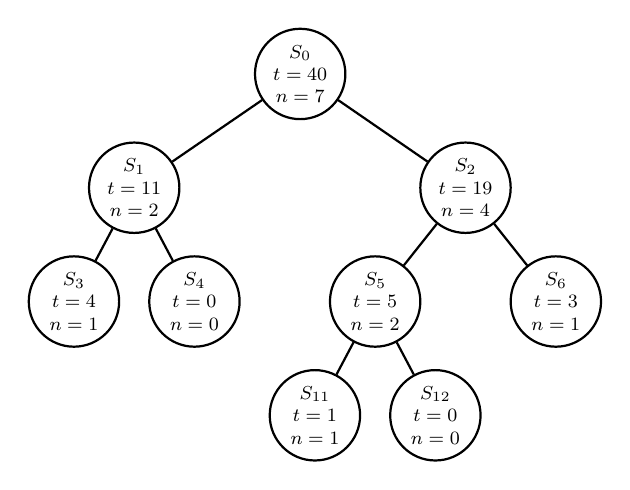
\begin{tikzpicture}[scale=0.85, every node/.style={transform shape}, mn/.style={draw, thick, circle, align=center, font=\footnotesize, inner sep=0.5pt, minimum size=13.5mm}]
\node[mn] (m1) at (3.38,0.00) {\textbf{$S_{0}$}\\ $t=40$\\ $n=7$};
\node[mn] (m2) at (0.90,-1.70) {\textbf{$S_{1}$}\\ $t=11$\\ $n=2$};
\node[mn] (m3) at (0.00,-3.40) {\textbf{$S_{3}$}\\ $t=4$\\ $n=1$};
\draw[thick] (m2) -- (m3);
\node[mn] (m4) at (1.80,-3.40) {\textbf{$S_{4}$}\\ $t=0$\\ $n=0$};
\draw[thick] (m2) -- (m4);
\draw[thick] (m1) -- (m2);
\node[mn] (m5) at (5.85,-1.70) {\textbf{$S_{2}$}\\ $t=19$\\ $n=4$};
\node[mn] (m6) at (4.50,-3.40) {\textbf{$S_{5}$}\\ $t=5$\\ $n=2$};
\node[mn] (m7) at (3.60,-5.10) {\textbf{$S_{11}$}\\ $t=1$\\ $n=1$};
\draw[thick] (m6) -- (m7);
\node[mn] (m8) at (5.40,-5.10) {\textbf{$S_{12}$}\\ $t=0$\\ $n=0$};
\draw[thick] (m6) -- (m8);
\draw[thick] (m5) -- (m6);
\node[mn] (m9) at (7.20,-3.40) {\textbf{$S_{6}$}\\ $t=3$\\ $n=1$};
\draw[thick] (m5) -- (m9);
\draw[thick] (m1) -- (m5);
\end{tikzpicture}
\end{adjustbox}
\end{center}
\end{solbox}
\subq{(b)}Which action is recommended at the root by the \emph{max child} rule, and which by the \emph{robust child} rule?
\begin{solbox}
Averages: $S_1$: $11/2=5.5$, $S_2$: $19/4=4.75$ $\Rightarrow$ max child \textbf{$S_1$}. Visits: $S_1$: 2, $S_2$: 4 $\Rightarrow$ robust child \textbf{$S_2$}. The rules disagree, so max-robust would continue the search.
\end{solbox}
\question{7}This problem is about map colouring. Each region must be coloured Red (R), Green (G) or Blue (B), and neighbouring regions must have different colours. The constraint graph is shown below. The following questions are mutually independent.\begin{center}
\begin{adjustbox}{max width=\linewidth}
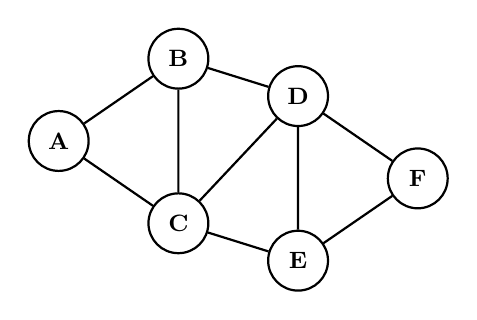
\begin{tikzpicture}[scale=0.95, every node/.style={transform shape}, cv/.style={draw, thick, circle, minimum size=8mm, inner sep=0pt, font=\small\bfseries}]
\node[cv] (A) at (0.00,1.00) {A};
\node[cv] (B) at (1.60,2.10) {B};
\node[cv] (C) at (1.60,-0.10) {C};
\node[cv] (D) at (3.20,1.60) {D};
\node[cv] (E) at (3.20,-0.60) {E};
\node[cv] (F) at (4.80,0.50) {F};
\draw[thick] (A) to[] (B);
\draw[thick] (A) to[] (C);
\draw[thick] (B) to[] (C);
\draw[thick] (B) to[] (D);
\draw[thick] (C) to[] (D);
\draw[thick] (C) to[] (E);
\draw[thick] (D) to[] (E);
\draw[thick] (D) to[] (F);
\draw[thick] (E) to[] (F);
\end{tikzpicture}
\end{adjustbox}
\end{center}
\subq{(a)}\textbf{Cross out} all values that would be eliminated by \emph{forward checking} after variable B has been assigned as shown.\begin{center}\small\begin{tabular}{|l|c|c|c|c|c|c|}\hline Variables & \textbf{A} & \textbf{B} & \textbf{C} & \textbf{D} & \textbf{E} & \textbf{F}\\ \hline Domains & R\ G\ B & \textbf{R} & R\ G\ B & R\ G\ B & R\ G\ B & R\ G\ B\\ \hline\end{tabular}\end{center}
\begin{solbox}
\begin{center}\small\begin{tabular}{|l|c|c|c|c|c|c|}\hline Variables & \textbf{A} & \textbf{B} & \textbf{C} & \textbf{D} & \textbf{E} & \textbf{F}\\ \hline Domains & \textcolor{red!70!black}{\sout{R}}\ G\ B & \textbf{R}\ \textcolor{red!70!black}{\sout{G}}\ \textcolor{red!70!black}{\sout{B}} & \textcolor{red!70!black}{\sout{R}}\ G\ B & \textcolor{red!70!black}{\sout{R}}\ G\ B & R\ G\ B & R\ G\ B\\ \hline\end{tabular}\end{center}Only the neighbours of B (A, C, D) lose R.
\end{solbox}
\subq{(b)}A and B have been assigned as shown, but no constraint propagation has been done yet. \textbf{Cross out} all values that would be eliminated by \emph{arc consistency} (AC-3).\begin{center}\small\begin{tabular}{|l|c|c|c|c|c|c|}\hline Variables & \textbf{A} & \textbf{B} & \textbf{C} & \textbf{D} & \textbf{E} & \textbf{F}\\ \hline Domains & \textbf{R} & \textbf{G} & R\ G\ B & R\ G\ B & R\ G\ B & R\ G\ B\\ \hline\end{tabular}\end{center}
\begin{solbox}
\begin{center}\small\begin{tabular}{|l|c|c|c|c|c|c|}\hline Variables & \textbf{A} & \textbf{B} & \textbf{C} & \textbf{D} & \textbf{E} & \textbf{F}\\ \hline Domains & \textbf{R}\ \textcolor{red!70!black}{\sout{G}}\ \textcolor{red!70!black}{\sout{B}} & \textcolor{red!70!black}{\sout{R}}\ \textbf{G}\ \textcolor{red!70!black}{\sout{B}} & \textcolor{red!70!black}{\sout{R}}\ \textcolor{red!70!black}{\sout{G}}\ B & R\ \textcolor{red!70!black}{\sout{G}}\ \textcolor{red!70!black}{\sout{B}} & \textcolor{red!70!black}{\sout{R}}\ G\ \textcolor{red!70!black}{\sout{B}} & \textcolor{red!70!black}{\sout{R}}\ \textcolor{red!70!black}{\sout{G}}\ B\\ \hline\end{tabular}\end{center}Propagation continues through the graph (unlike forward checking): every arc $X_i\to X_j$ is revised until no domain changes. Here arc consistency even leaves a single value for every variable.
\end{solbox}
\subq{(c)}Variable A is already assigned and constraint propagation has been done. \textbf{Circle} all unassigned variables that might be selected by the \emph{Minimum-Remaining-Values} (MRV) heuristic.\begin{center}\small\begin{tabular}{|l|c|c|c|c|c|c|}\hline Variables & \textbf{A} & \textbf{B} & \textbf{C} & \textbf{D} & \textbf{E} & \textbf{F}\\ \hline Domains & \textbf{R} & G\ B & G\ B & R\ G\ B & R\ G\ B & R\ G\ B\\ \hline\end{tabular}\end{center}
\begin{solbox}
Remaining values: B: 2, C: 2, D: 3, E: 3, F: 3 $\Rightarrow$ MRV may select \textbf{B, C}.
\end{solbox}
\subq{(d)}Same situation. \textbf{Circle} all unassigned variables that might be selected by the \emph{Degree Heuristic}.\begin{center}\small\begin{tabular}{|l|c|c|c|c|c|c|}\hline Variables & \textbf{A} & \textbf{B} & \textbf{C} & \textbf{D} & \textbf{E} & \textbf{F}\\ \hline Domains & \textbf{R} & G\ B & G\ B & R\ G\ B & R\ G\ B & R\ G\ B\\ \hline\end{tabular}\end{center}
\begin{solbox}
Degree = number of constraints with other \emph{unassigned} variables: B: 2, C: 3, D: 4, E: 3, F: 2 $\Rightarrow$ the degree heuristic may select \textbf{D}.
\end{solbox}
\subq{(e)}Assume no variable has been assigned yet. Solve the CSP using backtracking with \emph{forward checking}, choosing variables with MRV, then the degree heuristic (DH), and finally alphabetical order; try values in the order R, G, B. For every step give the MRV value of every region not yet coloured, and the DH values of the regions tied on the minimum MRV.
\begin{solbox}
\par \underline{Step 1}\par\begin{center}\small \begin{tabular}{|l|c|c|c|c|c|c|}\hline Variables & \textbf{A} & \textbf{B} & \textbf{C} & \textbf{D} & \textbf{E} & \textbf{F}\\ \hline MRV & \textcolor{blue!60!black}{3} & \textcolor{blue!60!black}{3} & \textcolor{blue!60!black}{3} & \textcolor{blue!60!black}{3} & \textcolor{blue!60!black}{3} & \textcolor{blue!60!black}{3}\\ \hline DH & \textcolor{blue!60!black}{2} & \textcolor{blue!60!black}{3} & \textcolor{blue!60!black}{4} & \textcolor{blue!60!black}{4} & \textcolor{blue!60!black}{3} & \textcolor{blue!60!black}{2}\\ \hline\end{tabular}\end{center}Assign to the variable \textbf{C} with the value \textbf{R} (tie on MRV and DH, broken alphabetically). Domains before this step: A=RGB, B=RGB, C=RGB, D=RGB, E=RGB, F=RGB.\par
\underline{Step 2}\par\begin{center}\small \begin{tabular}{|l|c|c|c|c|c|c|}\hline Variables & \textbf{A} & \textbf{B} & \textbf{C} & \textbf{D} & \textbf{E} & \textbf{F}\\ \hline MRV & \textcolor{blue!60!black}{2} & \textcolor{blue!60!black}{2} & -- & \textcolor{blue!60!black}{2} & \textcolor{blue!60!black}{2} & \textcolor{blue!60!black}{3}\\ \hline DH & \textcolor{blue!60!black}{1} & \textcolor{blue!60!black}{2} &  & \textcolor{blue!60!black}{3} & \textcolor{blue!60!black}{2} & \\ \hline\end{tabular}\end{center}Assign to the variable \textbf{D} with the value \textbf{G} (tie on MRV broken by DH). Domains before this step: A=GB, B=GB, C=R, D=GB, E=GB, F=RGB.\par
\underline{Step 3}\par\begin{center}\small \begin{tabular}{|l|c|c|c|c|c|c|}\hline Variables & \textbf{A} & \textbf{B} & \textbf{C} & \textbf{D} & \textbf{E} & \textbf{F}\\ \hline MRV & \textcolor{blue!60!black}{2} & \textcolor{blue!60!black}{1} & -- & -- & \textcolor{blue!60!black}{1} & \textcolor{blue!60!black}{2}\\ \hline DH &  & \textcolor{blue!60!black}{1} &  &  & \textcolor{blue!60!black}{1} & \\ \hline\end{tabular}\end{center}Assign to the variable \textbf{B} with the value \textbf{B} (tie on MRV and DH, broken alphabetically). Domains before this step: A=GB, B=B, C=R, D=G, E=B, F=RB.\par
\underline{Step 4}\par\begin{center}\small \begin{tabular}{|l|c|c|c|c|c|c|}\hline Variables & \textbf{A} & \textbf{B} & \textbf{C} & \textbf{D} & \textbf{E} & \textbf{F}\\ \hline MRV & \textcolor{blue!60!black}{1} & -- & -- & -- & \textcolor{blue!60!black}{1} & \textcolor{blue!60!black}{2}\\ \hline DH & \textcolor{blue!60!black}{0} &  &  &  & \textcolor{blue!60!black}{1} & \\ \hline\end{tabular}\end{center}Assign to the variable \textbf{E} with the value \textbf{B} (tie on MRV broken by DH). Domains before this step: A=G, B=B, C=R, D=G, E=B, F=RB.\par
\underline{Step 5}\par\begin{center}\small \begin{tabular}{|l|c|c|c|c|c|c|}\hline Variables & \textbf{A} & \textbf{B} & \textbf{C} & \textbf{D} & \textbf{E} & \textbf{F}\\ \hline MRV & \textcolor{blue!60!black}{1} & -- & -- & -- & -- & \textcolor{blue!60!black}{1}\\ \hline DH & \textcolor{blue!60!black}{0} &  &  &  &  & \textcolor{blue!60!black}{0}\\ \hline\end{tabular}\end{center}Assign to the variable \textbf{A} with the value \textbf{G} (tie on MRV and DH, broken alphabetically). Domains before this step: A=G, B=B, C=R, D=G, E=B, F=R.\par
\underline{Step 6}\par\begin{center}\small \begin{tabular}{|l|c|c|c|c|c|c|}\hline Variables & \textbf{A} & \textbf{B} & \textbf{C} & \textbf{D} & \textbf{E} & \textbf{F}\\ \hline MRV & -- & -- & -- & -- & -- & \textcolor{blue!60!black}{1}\\ \hline DH &  &  &  &  &  & \\ \hline\end{tabular}\end{center}Assign to the variable \textbf{F} with the value \textbf{R} (unique minimum MRV). Domains before this step: A=G, B=B, C=R, D=G, E=B, F=R.\par Solution: A=G, B=B, C=R, D=G, E=B, F=R. No backtracking is needed.
\end{solbox}
\question{8}\textit{Planning a study session.} You are planning a study session with four decisions: the (S)ubject, the (P)lace, the (T)ime and the (F)ood. The candidates are S $\in\{$\emph{ai, math, phys}$\}$, P $\in\{$\emph{library, cafe, home}$\}$, T $\in\{$\emph{morning, afternoon, evening}$\}$, F $\in\{$\emph{pizza, salad, noodles}$\}$, with the constraints: (1) the library is open only in the morning or afternoon; (2) math must be studied in the morning; (3) pizza is not allowed in the library; (4) AI cannot be studied at the cafe (no sockets).
\subq{(a)}Formulate the problem as a CSP: variables, domains and binary constraints.
\begin{solbox}
\begin{center}\small\begin{tabular}{|l|c|c|c|c|}\hline Variables & \textbf{S} & \textbf{P} & \textbf{T} & \textbf{F}\\ \hline Domains & ai, math, phys & library, cafe, home & morning, afternoon, evening & pizza, salad, noodles\\ \hline\end{tabular}\end{center}Binary constraints: (1) between P and T, (2) between S and T, (3) between P and F, (4) between S and P.
\end{solbox}
\subq{(b)}Draw the constraint graph.
\begin{solbox}
\begin{center}
\begin{adjustbox}{max width=\linewidth}
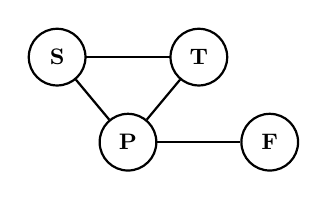
\begin{tikzpicture}[scale=0.9, every node/.style={transform shape}, cv/.style={draw, thick, circle, minimum size=8mm, inner sep=0pt, font=\small\bfseries}]
\node[cv] (S) at (0.00,1.20) {S};
\node[cv] (T) at (2.00,1.20) {T};
\node[cv] (P) at (1.00,0.00) {P};
\node[cv] (F) at (3.00,0.00) {F};
\draw[thick] (S) to[] (T);
\draw[thick] (S) to[] (P);
\draw[thick] (P) to[] (T);
\draw[thick] (P) to[] (F);
\end{tikzpicture}
\end{adjustbox}
\end{center}
\end{solbox}
\subq{(c)}You decide to study in the \emph{evening}. Cross out the eliminated values to show the domains after arc consistency has been enforced.
\begin{solbox}
\begin{center}\small\begin{tabular}{|l|c|c|c|c|}\hline Variables & \textbf{S} & \textbf{P} & \textbf{T} & \textbf{F}\\ \hline Domains & ai\ \textcolor{red!70!black}{\sout{math}}\ phys & \textcolor{red!70!black}{\sout{library}}\ cafe\ home & \textcolor{red!70!black}{\sout{morning}}\ \textcolor{red!70!black}{\sout{afternoon}}\ \textbf{evening} & pizza\ salad\ noodles\\ \hline\end{tabular}\end{center}(1) removes \emph{library}; (2) removes \emph{math}; then no other arc can remove anything: \emph{ai} still has support \emph{home}, and \emph{pizza} has support \emph{cafe}/\emph{home}.
\end{solbox}
\subq{(d)}Give one solution, or state that none exists.
\begin{solbox}
For example S=ai, P=home, T=evening, F=pizza (there are 9 solutions with T=evening).
\end{solbox}
\question{9}Answer the following questions briefly.
\subq{(a)}Russell \& Norvig organise definitions of AI into four categories. Name them, state which one this course adopts and give two reasons.
\begin{solbox}
Thinking humanly (cognitive modelling), thinking rationally (laws of thought), acting humanly (Turing test), acting rationally (\textbf{rational agent} --- adopted). Reasons: it is more general than the laws-of-thought approach (correct inference is only one way to act rationally; sometimes something must be done with no provably correct choice), and rationality is mathematically well defined, so it is more amenable to scientific development than approaches based on human behaviour or thought.
\end{solbox}
\subq{(b)}Explain the difference between the state space and the search tree, and between tree-search and graph-search algorithms.
\begin{solbox}
The state space is the graph of world states and actions (each state once). The search tree contains paths from the initial state; a state may appear in many nodes. Tree-search does not check redundant paths; graph-search keeps a \emph{reached} table and only the best path to each state. Tree-search suits formulations where redundant paths are rare, or when memory is too small for the reached table.
\end{solbox}
\subq{(c)}For a uniform tree with branching factor $b=5$ and the shallowest goal at depth $d=4$, how many nodes does BFS generate in the worst case? Why is memory a bigger problem than time for BFS?
\begin{solbox}
$b+b^2+b^3+b^4=5+25+125+625=\mathbf{780}$. All generated nodes stay in memory ($O(b^d)$ space as well as time), and memory is exhausted long before the time limit (lecture table: terabytes needed at depth 10--12).
\end{solbox}
\subq{(d)}Name three landscape features on which hill climbing gets stuck. If one run succeeds with probability $p=0.14$, how many restarts does random-restart hill climbing need on average?
\begin{solbox}
Local maxima, ridges, plateaux (flat local maxima / shoulders). Expected restarts $1/p\approx\mathbf{7}$.
\end{solbox}
\subq{(e)}Why should variable selection in backtracking be fail-first while value selection is fail-last?
\begin{solbox}
All variables must be assigned anyway, so a doomed branch should fail as early as possible (MRV/degree prune big subtrees). For values we need only one solution, so we try the value most likely to succeed (LCV keeps the most options for the neighbours).
\end{solbox}
\question{10}True or false?
For each statement, circle \textbf{T} or \textbf{F} and justify your answer in one or two sentences (an answer without a correct justification earns no credit).
\subq{1.}BFS is cost-optimal whenever all action costs are strictly positive. \hfill \textbf{T \quad F}
\begin{solbox}
\F. BFS returns the shallowest goal; it is optimal only when all step costs are equal (e.g.\ $S\to G$ costing 10 vs $S\to A\to G$ costing 2).
\end{solbox}
\subq{2.}Uniform-cost search applies the goal test when a node is generated. \hfill \textbf{T \quad F}
\begin{solbox}
\F. It tests when the node is removed from the frontier; testing at generation could return a more expensive path.
\end{solbox}
\subq{3.}Every consistent heuristic is admissible. \hfill \textbf{T \quad F}
\begin{solbox}
\T. Summing $h(n_i)\le c(n_i,n_{i+1})+h(n_{i+1})$ along an optimal path gives $h(n)\le h^*(n)$ since $h(\text{goal})=0$.
\end{solbox}
\subq{4.}If $h_1$ and $h_2$ are admissible, then $\max\{h_1,h_2\}$ is admissible and dominates both. \hfill \textbf{T \quad F}
\begin{solbox}
\T. At each node it equals one of two lower bounds, and it is $\ge$ each of them by definition.
\end{solbox}
\subq{5.}Greedy best-first (graph) search is complete in infinite state spaces. \hfill \textbf{T \quad F}
\begin{solbox}
\F. Only in finite spaces; in an infinite space it can follow an infinite path along which $h$ keeps decreasing.
\end{solbox}
\subq{6.}A poor move ordering may make alpha-beta return a different root value than minimax. \hfill \textbf{T \quad F}
\begin{solbox}
\F. Alpha-beta prunes only branches that cannot affect the decision; ordering changes only how much is pruned.
\end{solbox}
\subq{7.}With perfect move ordering alpha-beta examines $O(b^{m/2})$ nodes. \hfill \textbf{T \quad F}
\begin{solbox}
\T. The effective branching factor becomes $\sqrt b$, so it can search about twice as deep as minimax in the same time.
\end{solbox}
\subq{8.}In MCTS with UCB1, once a node has children, each of them is selected at least once before any of them is selected a second time. \hfill \textbf{T \quad F}
\begin{solbox}
\T. An unvisited child has UCB1 $=\infty$.
\end{solbox}
\subq{9.}Forward checking detects every inconsistency that arc consistency detects. \hfill \textbf{T \quad F}
\begin{solbox}
\F. FC only prunes neighbours of the variable just assigned; it misses conflicts between two unassigned variables, which AC propagates.
\end{solbox}
\subq{10.}In simulated annealing a worse move ($\Delta E<0$) is accepted with probability $e^{\Delta E/T}$, which decreases as $T$ decreases. \hfill \textbf{T \quad F}
\begin{solbox}
\T. E.g.\ $\Delta E=-2$: $T=4\Rightarrow 0.61$, $T=1\Rightarrow0.14$.
\end{solbox}
\end{document}